%% abtex2-modelo-trabalho-academico.tex, v-1.9.7 laurocesar
%% Copyright 2012-2018 by abnTeX2 group at http://www.abntex.net.br/ 
%%
%% This work may be distributed and/or modified under the
%% conditions of the LaTeX Project Public License, either version 1.3
%% of this license or (at your option) any later version.
%% The latest version of this license is in
%%   http://www.latex-project.org/lppl.txt
%% and version 1.3 or later is part of all distributions of LaTeX
%% version 2005/12/01 or later.
%%
%% This work has the LPPL maintenance status `maintained'.
%% 
%% The Current Maintainer of this work is the abnTeX2 team, led
%% by Lauro César Araujo. Further information are available on 
%% http://www.abntex.net.br/
%%
%% This work consists of the files abntex2-modelo-trabalho-academico.tex,
%% abntex2-modelo-include-comandos and abntex2-modelo-references.bib
%%

% ------------------------------------------------------------------------
% ------------------------------------------------------------------------
% abnTeX2: Modelo de Trabalho Academico (tese de doutorado, dissertacao de
% mestrado e trabalhos monograficos em geral) em conformidade com 
% ABNT NBR 14724:2011: Informacao e documentacao - Trabalhos academicos -
% Apresentacao
% ------------------------------------------------------------------------
% ------------------------------------------------------------------------

\documentclass[
	% -- opções da classe memoir --
	12pt,				% tamanho da fonte
	%openright,			% capítulos começam em pág ímpar (insere página vazia caso preciso)
	oneside,			% para impressão em recto e verso. Oposto a oneside
	a4paper,			% tamanho do papel. 
	% -- opções da classe abntex2 --
	chapter=TITLE,		% títulos de capítulos convertidos em letras maiúsculas
	%section=TITLE,		% títulos de seções convertidos em letras maiúsculas
	%subsection=TITLE,	% títulos de subseções convertidos em letras maiúsculas
	%subsubsection=TITLE,% títulos de subsubseções convertidos em letras maiúsculas
	% -- opções do pacote babel --
	english,			% idioma adicional para hifenização
	french,				% idioma adicional para hifenização
	spanish,			% idioma adicional para hifenização
	brazil				% o último idioma é o principal do documento
	]{abntex2}

% ---
% Pacotes básicos 
% ---
\usepackage{lmodern}			% Usa a fonte Latin Modern			
\usepackage[T1]{fontenc}		% Selecao de codigos de fonte.
\usepackage[utf8]{inputenc}		% Codificacao do documento (conversão automática dos acentos)
\usepackage{indentfirst}		% Indenta o primeiro parágrafo de cada seção.
\usepackage{color}				% Controle das cores
\usepackage{graphicx}			% Inclusão de gráficos
\usepackage{microtype} 			% para melhorias de justificação
\usepackage{float}
\usepackage{array}
\usepackage{multicol}
\usepackage{amsmath}
\usepackage{minted}
\usepackage{subfig}
\usepackage{subfigure}
% ---
		
% ---
% Pacotes adicionais, usados apenas no âmbito do Modelo Canônico do abnteX2
% ---
\usepackage{lipsum}				% para geração de dummy text
% ---

% ---
% Pacotes de citações
% ---
\usepackage[brazilian,hyperpageref]{backref}	 % Paginas com as citações na bibl
\usepackage[alf]{abntex2cite}	% Citações padrão ABNT

% --- 
% CONFIGURAÇÕES DE PACOTES
% --- 
\graphicspath{ {images/} } %definindo localização das imagens
% ---
% Configurações do pacote backref
% Usado sem a opção hyperpageref de backref
\renewcommand{\backrefpagesname}{Citado na(s) página(s):~}
% Texto padrão antes do número das páginas
\renewcommand{\backref}{}
% Define os textos da citação
\renewcommand*{\backrefalt}[4]{
	\ifcase #1 %
		Nenhuma citação no texto.%
	\or
		Citado na página #2.%
	\else
		Citado #1 vezes nas páginas #2.%
	\fi}%
% ---

% ---
% Informações de dados para CAPA e FOLHA DE ROSTO
% ---
\titulo{Sistema de Recomendação para Técnicas de Tolerância a Falhas em Ambientes de Nuvem}
\autor{Pedrenrique Gonçalves Guimarães}
\local{São José do Rio Preto, SP}
\data{2019}
\orientador{Aleardo Manacero Junior}
\instituicao{%
  Universidade Estadual Paulista ``Júlio de Mesquita Filho'' (UNESP)
  \par
  Instituto de Biociências, Letras e Ciências Exatas (IBILCE)
  \par
  Departamento de Ciências de Computação e Estatística}
\tipotrabalho{Tese (Graduação)}
% O preambulo deve conter o tipo do trabalho, o objetivo, 
% o nome da instituição e a área de concentração 
\preambulo{Trabalho de Conclusão de Curso (TCC) apresentado como parte dos requisitos para obtenção do título de Bacharel em Ciência da Computação, junto ao Departamento de Ciência da Computação e Estatística, do Instituto de Biociências, Letras e Ciências Exatas da Universidade Estadual Paulista “Júlio de Mesquita Filho”, Câmpus de São José do Rio Preto.}
% ---


% ---
% Configurações de aparência do PDF final

% alterando o aspecto da cor azul
\definecolor{blue}{RGB}{41,5,195}

% informações do PDF
\makeatletter
\hypersetup{
     	%pagebackref=true,
		pdftitle={\@title}, 
		pdfauthor={\@author},
    	pdfsubject={\imprimirpreambulo},
	    pdfcreator={LaTeX with abnTeX2},
		pdfkeywords={abnt}{latex}{abntex}{abntex2}{trabalho acadêmico}, 
		colorlinks=true,       		% false: boxed links; true: colored links
    	linkcolor=blue,          	% color of internal links
    	citecolor=blue,        		% color of links to bibliography
    	filecolor=magenta,      		% color of file links
		urlcolor=blue,
		bookmarksdepth=4
}
\makeatother
% --- 

% ---
% Posiciona figuras e tabelas no topo da página quando adicionadas sozinhas
% em um página em branco. Ver https://github.com/abntex/abntex2/issues/170
\makeatletter
\setlength{\@fptop}{5pt} % Set distance from top of page to first float
\makeatother
% ---

% ---
% Possibilita criação de Quadros e Lista de quadros.
% Ver https://github.com/abntex/abntex2/issues/176
%
\newcommand{\quadroname}{Quadro}
\newcommand{\listofquadrosname}{Lista de quadros}

%\newfloat[chapter]{quadro}{loq}{\quadroname}
\newlistof{listofquadros}{loq}{\listofquadrosname}
\newlistentry{quadro}{loq}{0}

% configurações para atender às regras da ABNT
\setfloatadjustment{quadro}{\centering}
\counterwithout{quadro}{chapter}
\renewcommand{\cftquadroname}{\quadroname\space} 
\renewcommand*{\cftquadroaftersnum}{\hfill--\hfill}

\setfloatlocations{quadro}{hbtp} % Ver https://github.com/abntex/abntex2/issues/176
% ---

% --- 
% Espaçamentos entre linhas e parágrafos 
% --- 

% O tamanho do parágrafo é dado por:
\setlength{\parindent}{1.3cm}

% Controle do espaçamento entre um parágrafo e outro:
\setlength{\parskip}{0.2cm}  % tente também \onelineskip

% ---
% compila o indice
% ---
\makeindex
% ---

% ----
% Início do documento
% ----
\begin{document}

% Seleciona o idioma do documento (conforme pacotes do babel)
%\selectlanguage{english}
\selectlanguage{brazil}

% Retira espaço extra obsoleto entre as frases.
\frenchspacing 

% ----------------------------------------------------------
% ELEMENTOS PRÉ-TEXTUAIS
% ----------------------------------------------------------
% \pretextual

% ---
% Capa
% ---
\imprimircapa
% ---

% ---
% Folha de rosto
% (o * indica que haverá a ficha bibliográfica)
% ---
\imprimirfolhaderosto*
% ---

% ---
% Inserir a ficha bibliografica
% ---

% Isto é um exemplo de Ficha Catalográfica, ou ``Dados internacionais de
% catalogação-na-publicação''. Você pode utilizar este modelo como referência. 
% Porém, provavelmente a biblioteca da sua universidade lhe fornecerá um PDF
% com a ficha catalográfica definitiva após a defesa do trabalho. Quando estiver
% com o documento, salve-o como PDF no diretório do seu projeto e substitua todo
% o conteúdo de implementação deste arquivo pelo comando abaixo:
%
% \begin{fichacatalografica}
%     \includepdf{fig_ficha_catalografica.pdf}
% \end{fichacatalografica}

\begin{fichacatalografica}
	\sffamily
	\vspace*{\fill}					% Posição vertical
	\begin{center}					% Minipage Centralizado
	\fbox{\begin{minipage}[c][8cm]{13.5cm}		% Largura
	\small
	\imprimirautor
	%Sobrenome, Nome do autor
	
	\hspace{0.5cm} \imprimirtitulo  / \imprimirautor. --
	\imprimirlocal, \imprimirdata-
	
	\hspace{0.5cm} \thelastpage p. : il. (algumas color.) ; 30 cm.\\
	
	\hspace{0.5cm} \imprimirorientadorRotulo~\imprimirorientador\\
	
	\hspace{0.5cm}
	\parbox[t]{\textwidth}{\imprimirtipotrabalho~--~\imprimirinstituicao,
	\imprimirdata.}\\
	
	\hspace{0.5cm}
		1. Computação em nuvem.
		2. Tolerância a falhas.
		2. Sistema de recomendação.
		I. Aleardo Manacero Junior.
		II. Universidade Estadual Paulista ``Júlio de Mesquita Filho'' - UNESP.
		III. Departamento de Ciência da Computação e Estatística.
		IV. Bacharelado em Ciência da Computação 			
	\end{minipage}}
	\end{center}
\end{fichacatalografica}
% ---

% ---
% Inserir errata
% ---
%\begin{errata}
%Elemento opcional da \citeonline[4.2.1.2]{NBR14724:2011}. Exemplo:
%
%\vspace{\onelineskip}

%FERRIGNO, C. R. A. \textbf{Tratamento de neoplasias ósseas apendiculares com
%reimplantação de enxerto ósseo autólogo autoclavado associado ao plasma
%rico em plaquetas}: estudo crítico na cirurgia de preservação de membro em
%cães. 2011. 128 f. Tese (Livre-Docência) - Faculdade de Medicina Veterinária e
%Zootecnia, Universidade de São Paulo, São Paulo, 2011.

%\begin{table}[htb]
%\center
%\footnotesize
%\begin{tabular}{|p{1.4cm}|p{1cm}|p{3cm}|p{3cm}|}
%  \hline
%   \textbf{Folha} & \textbf{Linha}  & \textbf{Onde se lê}  & \textbf{Leia-se}  \\
%    \hline
%    1 & 10 & auto-conclavo & autoconclavo\\
%   \hline
%\end{tabular}
%\end{table}
%
%\end{errata}
% ---

% ---
% Inserir folha de aprovação
% ---

% Isto é um exemplo de Folha de aprovação, elemento obrigatório da NBR
% 14724/2011 (seção 4.2.1.3). Você pode utilizar este modelo até a aprovação
% do trabalho. Após isso, substitua todo o conteúdo deste arquivo por uma
% imagem da página assinada pela banca com o comando abaixo:
%
% \begin{folhadeaprovacao}
% \includepdf{folhadeaprovacao_final.pdf}
% \end{folhadeaprovacao}
%
\begin{folhadeaprovacao}

  \begin{center}
    {\ABNTEXchapterfont\large\imprimirautor}

    \vspace*{\fill}\vspace*{\fill}
    \begin{center}
      \ABNTEXchapterfont\bfseries\Large\imprimirtitulo
    \end{center}
    \vspace*{\fill}
    
    \hspace{.45\textwidth}
    \begin{minipage}{.5\textwidth}
        \imprimirpreambulo
    \end{minipage}%
    \vspace*{\fill}
   \end{center}
        
   Trabalho aprovado. \imprimirlocal, %24 de novembro de 2012:

   \assinatura{\textbf{\imprimirorientador} \\ UNESP – Câmpus de São José do Rio Preto \\ Orientador} 
   \assinatura{\textbf{Renata Spolon Lobato} \\ UNESP – Câmpus de São José do Rio Preto}
   \assinatura{\textbf{Rodrigo Capobianco Guido} \\ UNESP – Câmpus de São José do Rio Preto}
   %\assinatura{\textbf{Professor} \\ Convidado 3}
   %\assinatura{\textbf{Professor} \\ Convidado 4}
      
   \begin{center}
    \vspace*{0.5cm}
    {\large\imprimirlocal}
    \par
    {\large\imprimirdata}
    \vspace*{1cm}
  \end{center}
  
\end{folhadeaprovacao}
% ---

% ---
% Dedicatória
% ---

\begin{dedicatoria}
   \vspace*{\fill}
   \centering
   \noindent
   \textit{Dedico este trabalho ao meu avô Lucrécio (in memorian), \\ que desde o começo de minha jornada fez questão de declarar seu absoluto apoio, \\ e que agora descansa na mais perfeita confusão.} \vspace*{\fill}
\end{dedicatoria}
% ---

% ---
% Agradecimentos
% ---
%\begin{agradecimentos}
%
%
%\end{agradecimentos}
% ---

% ---
% Epígrafe
% ---
%\begin{epigrafe}
%    \vspace*{\fill}
%	\begin{flushright}
%		\textit{}
%	\end{flushright}
%\end{epigrafe}
% ---

% ---
% RESUMOS
% ---

% resumo em português
\setlength{\absparsep}{18pt} % ajusta o espaçamento dos parágrafos do resumo
\begin{resumo}
 A computação em nuvem tem ganhado grande popularidade nos últimos anos por oferecer uma gama de serviços e recursos diversificados de forma rápida, prática e bastante acessível para o público casual e também empresarial. Tais sistemas têm como principais características a escalabilidade e alta carga de trabalho, na maioria dos casos. Entretanto, as plataformas em nuvem também estão bastante suscetíveis a diversos tipos de falhas que podem comprometer o funcionamento dos serviçose e de toda sua infraestrutura, permitindo assim uma perda de dados massiva e possível interrupção de suas atividades por tempo indeterminado. Tais ambientes devem possuir uma boa tolerância a essas falhas, o que significa dizer que a equipe por trás desse ambiente deve ser capaz de identificar e resolver quaisquer falhas de forma a não deixar que estas comprometam o ambiente em questão. Para tratamento de tais falhas, existem diversas técnicas que buscam tratar tais problemas, incluindo uma sistematização em classes com as falhas mais comuns. Para auxiliar administradores desses serviço, este trabalho visa expandir tal sistematização, utilizando um sistema de recomendação inteligente que consiga fazer a sugestão das técnicas corretas para o tratamento de falhas no ambiente de forma automática.

 \textbf{Palavras-chave}: Computação em nuvem, tolerância a falhas, sistema de recomendação.
\end{resumo}

% resumo em inglês
\begin{resumo}[Abstract]
 \begin{otherlanguage*}{english}
   Cloud computing is gaining popularity in recent years for offering a variety of different services and resources in a quick, practical and very accessible way for the casual public and corporations. Such systems have the main characteristics the high scalabilty and workflow, in most cases. However, cloud platforms are also very susceptible to many different types of faults that may compromise the workings of the services and all of its infrastructure, allowing for a massive data loss and also possibly causing an unwanted interruption of its activities for some time. These services should be fault tolerant, which means that any potential failure that may happen during running time should not affect the system, and that the team behind it should be able to identify the problems and solve it without halting the entire operation of the service. There are several techniques available to treat these problems, including a systematic classification of most common faults. To help administrators of these services, this work aims to expand this classification, using an intelligent recommender system that is able to suggest the correct techniques to treat faults automatically.

   \vspace{\onelineskip}
 
   \noindent 
   \textbf{Keywords}: cloud computing, fault tolerance, recommender systems.
 \end{otherlanguage*}
\end{resumo}

% ---
% inserir lista de ilustrações
% ---
\pdfbookmark[0]{\listfigurename}{lof}
\listoffigures*
\cleardoublepage
% ---

% ---
% inserir lista de quadros
% ---
%\pdfbookmark[0]{\listofquadrosname}{loq}
%\listofquadros*
%\cleardoublepage
% ---

% ---
% inserir lista de tabelas
% ---
\pdfbookmark[0]{\listtablename}{lot}
\listoftables*
\cleardoublepage
% ---

% ---
% inserir lista de abreviaturas e siglas
% ---
%\begin{siglas}
%  \item[ABNT] Associação Brasileira de Normas Técnicas
%  \item[abnTeX] ABsurdas Normas para TeX
%\end{siglas}
% ---

% ---
% inserir lista de símbolos
% ---
%\begin{simbolos}
%  \item[$ \Gamma $] Letra grega Gama
%  \item[$ \Lambda $] Lambda
%  \item[$ \zeta $] Letra grega minúscula zeta
%  \item[$ \in $] Pertence
%\end{simbolos}
% ---

% ---
% inserir o sumario
% ---
\pdfbookmark[0]{\contentsname}{toc}
\tableofcontents*
\cleardoublepage
% ---



% ----------------------------------------------------------
% ELEMENTOS TEXTUAIS
% ----------------------------------------------------------
\textual

% ----------------------------------------------------------
% Introdução (exemplo de capítulo sem numeração, mas presente no Sumário)
% ----------------------------------------------------------
\chapter{Introdução}
% ----------------------------------------------------------
A computação em nuvem é uma forma de computação que provê diversos serviços distintos por meio da Internet, de forma que o usuário em questão possa acessar os serviços de qualquer plataforma, desde que possua uma conexão com a Internet. Esse tipo de computação tem se tornado muito popular com a expansão da rede mundial de computadores pelo mundo, e com o pesado investimento em infraestutura proporcionado pelas grandes corporações e operadoras de telecomunicações, que agora tornaram mais acessível ao usuário final o acesso a uma conexão rápida e estável, o que é um requisito fundamental para o correto funcionamento desses serviços.

Gigantes da computação como a Amazon, Google, IBM e Microsoft têm investido pesado em infraestrutura para oferecimento de serviços de computação em nuvem \cite{tsai2010service, lohr2007google}. Outras empresas ganharam grande notoriedade na indústria por oferecerem exclusivamente serviços de computação em nuvem, como é o caso da Netflix, Hulu e Dropbox, por exemplo \cite{berman2012cloud}. 

A alta demanda por tais serviços e modo de operação tem tornado cada vez mais comum o aparecimento de sistemas de computação em nuvem, e cada vez mais profissionais estão sendo treinados para serem capazes de desenvolver e manter tais tecnologias. Entretanto, não diferente de qualquer outro sistema computacional, sistemas de computação em nuvem também são bastante suscetíveis a diversos tipos de falhas e erros que podem comprometer o funcionamento do sistema como um todo. Cada tipo de falha pode ter uma origem diferente, com algum tipo de solução diferente, o que dificulta sua prevenção ou correção, dependendo do tipo de sistema utilizado. Diversos trabalhos na literatura abordam técnicas para lidar com tais falhas e previni-las, e propõem metodologias que visam classificar e identificar as melhores técnicas em casos específicos.

Este trabalho tem o intuito de acrescentar a essas metodologias uma forma de sugestão automática de técnicas de tolerância a falhas por meio de um sistema de recomendação, de forma com que a administração do sistema em questão possa focar na técnica sugerida em vez de buscar diversas soluções distintas que podem resultar em horas infrutíferas de trabalho.

\section{Motivação}

A crescente demanda por serviços baseados em nuvem tem feito o interesse pela área crescer entre os pesquisadores do âmbito da computação para lidar com a tolerância de falhas desses sistemas computacionais. Por consequência, o número de abordagens distintas para suprir tais falhas tem se multiplicado na literatura, e a escolha de abordagens envolve uma série de variáveis que podem levar a dúvidas com relação a qual destes métodos podem ser escolhidos durante uma situação real de risco. Nem sempre a escolha é a melhor possível para uma determinada situação, e uma abordagem pode ter diversos pontos negativos em sua execução.

Levando em conta que sistemas de computação em nuvem devem permanecer operantes de forma ininterrupta, a escolha dos melhores métodos de tolerância a falhas deve ser feita de forma inteligente e deve também estar sujeito a uma rigorosa avaliação por parte da equipe de administração.

\section{Objetivos}

Com o fato de haver inúmeras técnicas distintas para lidar com a tolerância de falhas nesses sistemas, cada uma com suas vantagens e desvantagens, a escolha dessas técnicas pode ser um processo difícil na contenção de falhas.

Utilizando um sistema de recomendação dessas abordagens, os administradores desses sistemas computacionais conseguem, de forma simples, escolher a melhor abordagem para suprir a situação, eliminando a necessidade de uma consulta mais aprofundada, o que, por sua vez, representa uma grande economia de tempo e esforço da equipe de administração.

\section{Organização do texto}

Este documento é dividido em capítulos, seções e diversas subseções. No capítulo a seguir (Capítulo \ref{cap_conceitos}), serão abordados os conceitos básicos necessários para o entendimento do trabalho. Os temas de computação em nuvem, tolerância a falhas e sistemas de recomendação serão analisados e explicados em suas respectivas seções.

Com os conceitos devidamente estabelecidos, o capítulo seguinte (Capítulo \ref{cap_projeto}), expõe as principais propostas para o projeto, com as devidas definições de implementação e detalhes necessários para tal.

No capítulo \ref{cap_testes} são executados os testes referentes ao funcionamento do sistema como um todo, buscando validar os recursos que o sistema se propõe a fazer. E, por fim, o capítulo \ref{cap_conclusão} faz a conclusão geral do que foi feito nesse trabalho, e algumas das perspectivas para uso futuro.
% ---
% Capitulo com exemplos de comandos inseridos de arquivo externo 
% ---
\include{abntex2-modelo-include-comandos}
% ---

\chapter{Fundamentação teórica}\label{cap_conceitos}

Como parte essencial para o entendimento do trabalho, este capítulo irá tratar dos principais conceitos e fundamentos necessários para a implementação do projeto de sistema de recomendação.

\section{Computação em nuvem}\label{sec_comp_nuv}

O termo computação em nuvem tem diferentes significados na literatura, e alguns exemplos podem ser mencionados. Em artigo publicado em \citeyear{fernando2013mobile}, \citeauthor{fernando2013mobile} afirmam que consumidores veem computação em nuvem como um serviço padronizado acessível por meio de um aparelho conectado à Internet. Por outro lado, outro artigo de \citeyear{mazhelis2012economic}, \citeauthor{mazhelis2012economic} alegam que profissionais de Tecnologia da Informação veem computação em nuvem como uma \emph{pool} de recursos compartilhados acessados por ambientes computacionais. \cite[p. 1]{khan2018cloud}

De uma forma geral, pode-se representar um exemplo de infraestrutura básica da computação em nuvem como definida na Figura \ref{fig:compnuvem}.

\begin{figure}[h]
	\caption{Exemplo de infraestrutura de computação em nuvem.}
	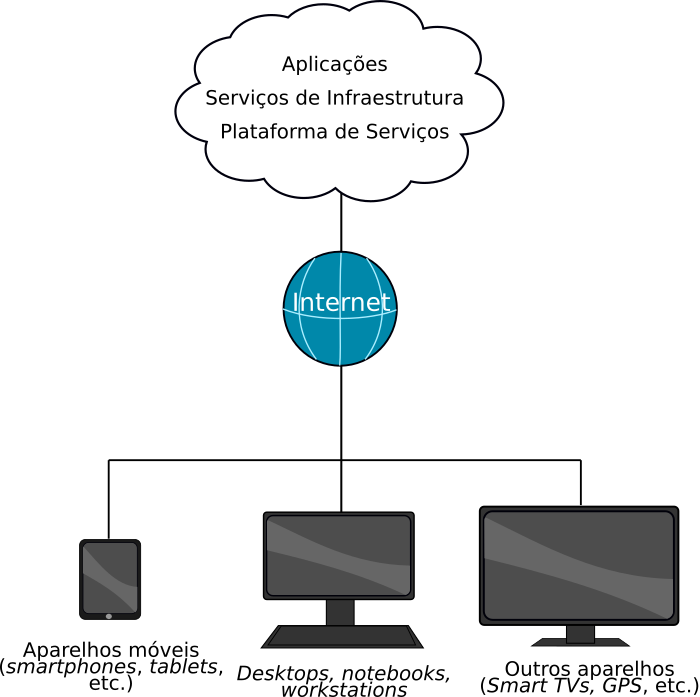
\includegraphics[scale=0.45]{compnuvem}
	\centering
	\label{fig:compnuvem}
	\\
	\centering \textual (Traduzido e adaptado pelo autor \cite{marston2011cloud})
\end{figure}

Em 2011, o \emph{Information Technology Laboratory} (ITL), que faz parte \emph{National Institute of Standards and Technology} (NIST), uma agência governamental que promove a utilização de padrões em ambientes de tecnologia da informação, lançou um documento que define a computação em nuvem como ``um modelo que permite acesso ubíquo, conveniente e sob demanda para uma gama de recursos computacionais compartilhados que podem ser provisionados e liberados com o mínimo de esforço ou interação do provedor de serviço.'' \cite[p. 2]{mell2011nist} (Tradução adaptada pelo autor).

O documento também prevê cinco características essenciais, três modelos de serviço e quatro modelos de implementação que definem o ambiente de computação em nuvem, que serão descritas nas subseções seguintes (\ref{caractessenciais}, \ref{modelosserv}, \ref{modelosimp}).

\subsection{Características essenciais}\label{caractessenciais}\label{sec_caracter}

O documento do NIST define as seguintes características essenciais para ambientes de computação em nuvem:
\begin{itemize}
	\item \textbf{Atendimento sob demanda:} O consumidor pode requisitar as operações do serviço em tempo real, como armazenamento de dados por exemplo, sem necessidade de interação humana com o provedor de serviços;
	\item \textbf{Amplo acesso à rede:} Os serviços são disponibilizados por meio do acesso à internet, utilizando mecanismos padronizados que permitam o acesso utilizando diferentes plataformas, como celulares, \emph{notebooks}, \emph{tablets}, \emph{desktops} etc;
	\item \textbf{\emph{Pool} de recursos:} Os recursos computacionais do provedor de serviços deve ser capaz de servir múltiplos consumidores ao mesmo tempo, com diferentes recursos físicos e virtuais sendo destinados dinamicamente de acordo com a demanda do consumidor;
	\item \textbf{Rápida elasticidade:} Os recursos computacionais podem ser fornecidos e liberados de forma elástica, em alguns casos de forma automática, escalando de forma adequada conforme a demanda. Para o consumidor, tais recursos podem parecer ilimitados, ou então podem ser adquiridos em qualquer quantidade a qualquer tempo;
	\item \textbf{Serviços mensuráveis:} Sistemas de nuvem controlam e otimizam automaticamente o uso de recursos utilizando recursos mensuráveis (que geralmente são alcançados utilizando um serviço de ``pagar por uso''). O uso de recursos pode ser monitorado, controlado, e reportado, promovendo transparência tanto para o consumidor quanto para o provedor de serviços.
\end{itemize}

\citeauthor{gong2010characteristics} (\citeyear{gong2010characteristics}) faz uma relação entre as características de computação em nuvem e computação em grade, um modelo computacional paralela que é baseada em alta performance computacional. Tal comparação está reproduzida na Tabela \ref{tab:comparacao}, de forma traduzida e adaptada.

\begin{table}[H]
    \ABNTEXchapterfont
    \centering
    \caption{Comparação entre Características de Computação em Nuvem e Computação em Grade}
    \begin{tabular}{|c|c|c|}
    \hline
        \textbf{Característica} & \textbf{Computação em nuvem}  & \textbf{Computação em grade}\\
        \hline
        \hline
        Orientada a Serviço & Sim  & Sim\\
        \hline
        Acoplamento Fraco & Sim  & Metade\\
        \hline
        Forte Tolerância a Falhas & Sim  & Metade\\
        \hline
        Modelo de negócios & Sim  & Não\\
        \hline
        Facilmente utilizável & Sim  & Metade \\
        \hline
        Baseado em TCP/IP & Sim & Metade\\
        \hline
        Alta segurança & Metade  & Metade\\
        \hline
        Virtualização & Sim  & Metade\\
    \hline
    \end{tabular}
    \label{tab:comparacao}
\end{table}

Na Tabela \ref{tab:comparacao}, os parâmetros ``sim'' e ``não'' referem-se à presença dessas características especiais nos sistemas, enquanto o parâmetro ``metade'' refere-se a uma presença parcial da característica no sistema computacional. Tal comparação é útil para diferenciar o fato de que Computação em Nuvem não necessariamente significa Computação de Alta Performance, embora muitas vezes estejam associados, e mostra claramente que existem diferenças claras entre os dois modelos computacionais.

Dessa forma, pode-se ver que existem características específicas do modelo de computação em nuvem que são bastante importantes para seu funcionamento.

\begin{itemize}
    \item \textbf{Orientado a serviço:} Serviços de computação em nuvem estão disponíveis para uso sob demanda, como descrito nas características essenciais;
    \item \textbf{Acoplamento fraco:} Ambientes de computação em nuvem utilizam-se de virtualização ou outras tecnologias que separam o lógico do físico. Na seção \ref{sec_arq_comp} isso será um pouco melhor explorado.
    \item \textbf{Forte tolerância a falhas:} Aspecto essencial deste trabalho, existem diversas publicações que mostram a importância da tolerância a falhas na computação em nuvem \cite{jhawar2012fault, ataallah2015fault, amin2015review, cheraghlou2016survey};
    \item \textbf{Modelo de negócios:} Característica chave que distingue computação em nuvem de computação em grade \cite[p. 278]{gong2010characteristics}. A computação em nuvem é fortemente suportada por grandes companhias na área de Tecnologia de Informação, e todas possuem lucro como principal objetivo do investimento nessas plataformas. Grande parte dos sistemas utiliza alguma forma de pagamento por uso de suas plataformas, e isso os torna sistemas bastante rentáveis para suas respectivas companhias.
\end{itemize}

\subsection{Modelos de serviço}\label{modelosserv}

Os modelos de serviço definidos no documento estão descritos a seguir, com tradução e adaptação pelo autor:

\begin{itemize}
	\item \textbf{\emph{Software as a Service (SaaS)}:} O recurso computacional é disponibilizado para o consumidor como uma aplicação executada em infraestrutura na nuvem. Essa aplicação pode ser acessada de diversos dispositivos, podendo-se utilizar um navegador de internet, ou até mesmo uma aplicação própria. O consumidor, neste caso, não tem nenhum controle sobre os servidores, sistemas operacionais, armazenamento ou aplicações que fazem parte da infraestrutura da rede, limitando-se apenas àquilo que lhe foi designado como serviço disponível;
	\item \textbf{\emph{Platform as a Service (PaaS)}:} O recurso disponibilizado ao consumidor é para a implementação de um sistema de computação em nuvem, podendo assim criar sua prórpia aplicação ou serviço utilizando a infraestrutura existente. Neste caso, o consumidor também não possui controle sobre tal infraestrutura, mas pode implementar aplicações e configurações no ambiente hospedeiro;
	\item \textbf{\emph{Infrastructure as a Service (IaaS)}:} O recurso computacional disponibilizado é prover processamento, armazenamento, rede e outros recursos fundamentais onde o consumidor pode implementar e executar sistemas operacionais e aplicações a seu gosto, quando disponíveis. O consumidor também não controla a infraestrutura, mas já tem controle sobre os sistemas operacionais, armazenamento e aplicações implementadas.
\end{itemize}

\subsection{Modelos de implementação}\label{modelosimp}

Os modelos de implementação mais comuns definidos pelo NIST são os modelos de nuvem privada, nuvem comunitária, nuvem pública e nuvem híbrida. As características de cada um desses serviços está descrita na Tabela \ref{tab:modelos}.

\begin{table}[ht]
\ABNTEXchapterfont
\centering

\caption{Modelos de Implementação de computação em nuvem}
\begin{tabular}{|m{3.8cm}|m{11.0cm}|}
    \hline
    \multicolumn{2}{|c|}{\centering\textbf{Modelos de Implementação}}\\
    \hline
    \hline
	\centering\textbf{Nuvem privada} & A infraestrutura em nuvem provisionada é de uso exclusivo de uma organização, compondo-se de múltiplos consumidores. \\
	\hline
	\centering\textbf{Nuvem comunitária} & A infraestrutura em nuvem provisionada é de uso exclusivo de uma comunidade específica de consumidores de organizações com interesses em comum.\\
	\hline
	\centering\textbf{Nuvem pública} & A infraestrutura em nuvem provisionada é aberta para o público em geral.\\
	\hline
	\centering\textbf{Nuvem híbrida} & A infraestrutura em nuvem disponibilizada é uma composição de duas ou mais infraestruturas de nuvem descritas anteriormente, que continuam operando de forma independente, mas que se interconectam por uma tecnologia padronizada que permite a portabilidade de aplicações e dados.\\
	\hline
	\end{tabular}
	\textual (Traduzido e adaptado pelo autor)
	\label{tab:modelos}
\end{table}


\subsection{Arquitetura de computação em nuvem}\label{sec_arq_comp}

De uma forma geral, podemos dividir a arquitetura de um sistema de computação em nuvem em quatro camadas \cite{zhang2010cloud}, como também visto na Figura \ref{fig:arqcompnuvem}:

\begin{itemize}
    \item \textbf{Camada de \emph{hardware}:} Responsável por gerenciar os recursos físicos da nuvem, como servidores, roteadores, \emph{switches}, energia e sistemas de resfriamento. Trata-se dos próprios \emph{data centers}.
    \item \textbf{Camada de infraestrutura:} Trata-se da camada de virtualização, que cria a \emph{pool} de armazenamento e recursos computacionais, particionando os recursos físicos usando tecnologias de virtualização.
    \item \textbf{Camada de plataforma:} Consiste no sistema operacional e nos \emph{frameworks} das aplicações. Essa camada facilita a implantação das aplicações executadas.
    \item \textbf{Camada de aplicação:} Consiste nas próprias aplicações executadas em nuvem. Nesses ambientes, as aplicações em nuvem podem ser escaláveis para obter melhor desempenho, acessibilidade e menor custo.
\end{itemize}

\begin{figure}[ht]
	\caption{Arquitetura da computação em nuvem.}
	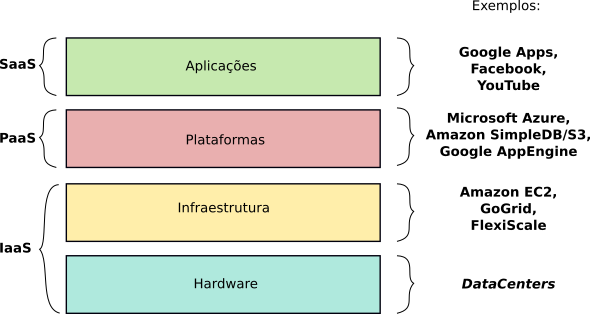
\includegraphics{images/arqcompnuvem.png}
	\centering
	\label{fig:arqcompnuvem}
	\textual (Traduzido e adaptado pelo autor)
\end{figure}

Tal arquitetura torna os serviços de computação em nuvem mais modulares quando comparados a tradicionais \emph{server farms}, por permitir que as camadas funcionem como módulos fracamente conectados entre si, permitindo que esses se expandam e evoluam de forma independente \cite[p. 9]{zhang2010cloud}.

\subsection{Aplicações na indústria}

Existem inúmeras aplicações de computação em nuvem na indústria, que variam de acordo com a natureza da indústria e sua carga de trabalho \cite[p. 10]{khan2018cloud}. Nesta seção, serão apresentados alguns serviços mais conhecidos e relevantes de computação em nuvem.

\subsubsection{\emph{Amazon Web Services (AWS)}}

Amazon Web Services (AWS) \cite{aws} é um conjunto de serviços de nuvem, que fornecem computação baseada em nuvem, armazenamento e outras aplicações que atendem tanto o aspecto corporativo quanto a usuários individuais. Nesse ambiente, usuários podem implementar aplicações e serviços sob demanda, pagando de acordo com o uso. \cite[p. 13]{zhang2010cloud}

Neste contexto, a Amazon disponibiliza também o serviço conhecido como \emph{\textbf{Amazon Elastic Compute Cloud}}, também chamado de \textbf{Amazon EC2}. Segundo o próprio serviço: ``O Amazon Elastic Compute Cloud (Amazon EC2) é um web service que disponibiliza capacidade computacional segura e redimensionável na nuvem. Ele foi projetado para facilitar a computação em nuvem na escala da web para os desenvolvedores.'' \cite{amazonec2}. Tal plataforma permite que o usuário administre servidores e \emph{data centers} utilizando APIs ou ferramentas e utilitários disponíveis. As instâncias da EC2 são máquinas virtuais sendo executadas dentro da engine de virtualização Xen \cite{xenengine, zhang2010cloud}.

A estrutura da AWS também comporta serviços como o Amazon Virtural Private Cloud (VPC), que se comporta como uma rede privada virtual (VPN), utilizando os recursos da AWS para permitir uma segurança adicional para o usuário final, com serviços de firewall, detecção de intrusão, entre outros serviços.

\subsubsection{Microsoft Azure}

A plataforma Microsoft Azure, antigamente chamada de Microsoft Windows Azure, consiste em uma plataforma da própria Microsoft para executar aplicações e armazenar dados na nuvem \cite{chappell2009introducing}.

Os serviços oferecidos são diversos: armazenamento de dados em nuvem, execução de aplicações, gerenciamento de contâineres, APIs de detecção facial, ferramentas de testes para desenvolvedores, entre outras aplicações \cite{microsoftazure}. 

\subsubsection{Dropbox}

Criado em 2007, o serviço conhecido como Dropbox \cite{dropbox} ocupa um nicho específico no ramo de computação em nuvem. Seu principal modelo de negócio é o armazenamento de dados em nuvem, oferecendo serviços para corporações e para usuários finais. Ele oferece aos usuários um serviço gratuito de armazenamento de até 2 GB por usuário. Esse montante pode ser expandido em até 3 TB ou mais mediante pagamento de planos específicos, que oferecem recursos adicionais como sincronização automática com dispositivos conectados, busca em texto, recuperação de arquivos desejados e suporte dedicado \cite{dropboxplans}.

\subsubsection{Google App Engine}

A Google App Engine é mais um dos serviços de computação em nuvem da Google. Consiste em uma plataforma para criação de aplicativos de forma escalonável, totalmente gerenciada e sem servidor. Na plataforma pode-se utilizar linguagens e frameworks populares como Java, PHP, Node.js, Python, C\#, .Net, Ruby e Go, ou o usuário pode também utilizar seu próprio framework sobre a plataforma \cite{googleapp}.

O serviço conta também com ferramentas para contâiners, controle de versão, segurança com certificados gerenciados SSL/TLS, ferramentas para depuração, dentre tantas outras opções para desenvolvedores.

\section{Tolerância a falhas}

O uso de sistemas computacionais é ubíquo no mundo moderno, extendendo-se a aplicações em sistemas de defesa, sistemas aéreo, controle de tráfego aéreo, sistemas bancários, jogos virtuais, dentre tantos outros. A variedade de aplicações e a importância crescente desse setor trouxe à tona a confiabilidade de sistemas computacionais para as mais diversas aplicações \cite{andersonfault}.

Um exemplo de preocupação com o funcionamento adequado desses sistemas ocorreu no fim da década de 1990, quando percebeu-se o modo ineficiente de armazenamento e formatação de datas de calendários em sistemas computacionais da época, e que colocaria em risco a correta execução de milhares de serviços dependentes desses sistemas, podendo também ocasionar uma pane geral de alguns sistemas de alto risco. Tal episódio é conhecido na literatura como ``Problema do Ano 2000'', muitas vezes estilizado como ``Y2K \emph{problem}'', ou popularmente chamado de ``\emph{Bug} do Milênio'' . A preocupação com uma pane em massa de praticamente todos os sistemas computacionais levou a criação de uma série de medidas para garantir a correção desse problema nos sistemas existentes e prevenir a ocorrência de problemas similares em futuros sistemas desenvolvidos \cite{petersen1998y2k}.

Este clássico exemplo de prevenção de falhas mostra uma fraqueza de alguns sistemas computacionais em lidar com falhas previstas anteriormente. Caso tais correções e recomendações não fossem consideradas, especula-se que as consequências poderiam ser catastróficas para os mais diversos setores que dependiam desses sistemas computacionais \cite{smith1997year}. Assim sendo, deve-se levar em consideração que existem problemas aos quais sistemas computacionais estão sujeitos, mas que podem ser tratados adequadamente em tempo de execução, evitando ao máximo comprometer o funcionamento desse sistema.

\subsection{Conceitos básicos}

Assim como os sistemas mencionados anteriormente estavam sujeitos a falhas causadas por uma falta de planejamento dos desenvolvedores, sistemas computacionais modernos também estão sujeitos a inúmeros tipos de falhas, que podem fugir completamente ao controle tanto de administradores do sistema quanto aos desenvolvedores ou fabricantes de tal produto.

Uma falha no sistema ocorre quando o serviço oferecido se desvia do serviço especificado, na qual o serviço especificado significa uma descrição coerente do que é esperado desse serviço. Nesse contexto, pode-se afirmar que ocorreu um erro, decorrente de uma falha. Isto é, o erro é uma manifestação de uma falha no sistema, e a falha é a manifestação do erro no serviço \cite{laprie1985dependable}.

O conceito de tolerância a falhas em computação é bastante antigo e se aplica tanto no âmbito do fabricante de \emph{hardware} quanto na área de desenvolvimento de \emph{software} \cite{randell1975system}. Para ambos, é importante garantir a confiabilidade do sistema para qualquer um que venha a utilizá-lo posteriormente. Isso quer dizer que o sistema deve garantir que, mesmo após a ocorrência de algum tipo de falha, não ocorra interrupções no serviço \cite{bala2012fault}. Assim como visto na seção \ref{sec_caracter}, tolerância a falhas é uma das principais características de um ambiente de computação em nuvem, e é objeto de estudo de diversos trabalhos na área.

A tolerância a falhas é pautada por processamento de erros, que se baseia em duas fases \cite{laprie1985dependable}:
\begin{enumerate}
    \item \textbf{Processamento de erro efetivo:} essa fase busca trazer o erro de volta ao estado latente, se possível a um estado anterior à ocorrência da falha;
    \item \textbf{Processamento de erro latente:} tenta garantir que o erro não se torne efetivo novamente.
\end{enumerate}

Entre os benefícios de se implementar tolerância a falhas na computação em nuvem estão inclusos: recuperação em situação de falha, baixo custo e melhora na métrica de desempenho \cite{patra2013fault}. No decorrer desta seção serão apresentadas algumas formas de como isso pode ser feito em um sistema de computação em nuvem.

\subsection{Métricas para Tolerância a Falhas}

\citeauthor{amin2015review} (\citeyear{amin2015review}) e \citeauthor{patra2013fault} (\citeyear{patra2013fault}) definem métricas para tolerância a falhas, que estão devidamente reproduzidas neste documento de forma traduzida e adaptada a seguir:

\begin{itemize}
        \item \textbf{Rendimento:}  Define o número de tarefas cuja execução foi concluída. O rendimento de um sistema deve ser alto;
        \item \textbf{Tempo de resposta:} O tempo que leva para um algoritmo responder deve ser minimizado;
        \item\textbf{Escalabilidade:} O número de nós do sistema não deve afetar a capacidade de tolerância a falhas do algoritmo;
        \item\textbf{Desempenho:} Parâmetro que mede a efetividade do sistema. O desempenho do sistema deve ser melhorado lentamente;
        \item\textbf{Disponibilidade:} Sua disponibilidade é diretamente proporcional a sua confiabilidade. Trata-se da possibilidade de que um item está funcional durante um determinado período de tempo;
        \item\textbf{Usabilidade:} Dá a dimensão do quanto um produto pode ser utilizado por um usuário para atingir seus objetivos com efetividade, eficiência e satisfação;
        \item\textbf{Confiabilidade:} Esse aspecto almeja dar o resultado correto ou aceitável durante um determinado período de tempo;
        \item\textbf{Sobrecarga associada:} Trata-se da sobrecarga resultante da implementação de um algoritmo. Sobrecargas podem ser impostas por conta de movimentos de tarefas entre processos ou uma comunicação entre processadores. Para a eficiência da técnica de tolerância a falhas, sobrecargas devem ser minimizadas;
        \item\textbf{Custo-benefício:} O custo neste quesito é apenas definido como custo de monitoramento.
\end{itemize}

\subsection{Técnicas de tolerância a falhas}

Existem diversas técnicas de tolerância a falhas descritas na literatura \cite{cheraghlou2016survey, ataallah2015fault, jhawar2012fault}. Essas técnicas podem ser classificadas em reativas ou proativas, no ambiente de computação em nuvem \cite{bala2012fault}. A seguir será apresentada uma visão geral das técnicas de tolerância a falhas no ambiente de computação em nuvem, sem levar em consideração plataformas específicas de computação em nuvem.

\subsubsection{Técnicas reativas}

Técnicas reativas de tolerância a falhas são utilizadas para reduzir o impacto dessas falhas em uma sitação em que elas de fato ocorreram \cite{bala2012fault, patra2013fault}. Assim sendo, segue uma descrição dessas técnicas:

\begin{itemize}
    \item \textbf{\emph{Check pointing/Restart:}} A tarefa em falha é reiniciada a partir do ponto de verificação mais recente. É uma técnica eficiente para grandes aplicações;
    \item \textbf{Replicação:} Executa várias réplicas da tarefa em diferentes recursos até que toda a tarefa replicada seja executada sem interrupções;
    \item \textbf{Migração de trabalho:} Mediante a ocorrência de falha, o trabalho é migrado para uma nova máquina;
    \item \textbf{\emph{S-Guard}:} É baseado em recuperação de \emph{rollback}, ou seja, desfazer e/ou descartar todas as alterações feitas durante determinada transação.
    \item \textbf{Reexecução:} É a técnica mais simples: reexecuta a tarefa no mesmo recurso de nuvem;
    \item \textbf{Ressubmissão de tarefa:} A tarefa em falha é submetida novamente para a mesma máquina na qual estava operando ou a uma máquina diferente;
    \item \textbf{Manipulação de exceções definidas pelo usuário:} Nesse caso o usuário define ações específicas da falha de tarefas para fluxos de trabalhos;
    \item \textbf{Resgate de fluxo de trabalho:} Permite que o sistema mantenha seu funcionamento após uma falha em qualquer tarefa até não ser mais capaz de prosseguir sem atender a tarefa falhada;
    \item \textbf{Reconfiguração:} Nesse procedimento é eliminado o componente em falha.
\end{itemize}

\subsubsection{Técnicas proativas}

No caso de técnicas proativas, elas são responsáveis por prever as falhas e substituir componentes suspeitos por outros componentes de trabalho. Nesse caso temos \cite{bala2012fault, patra2013fault}:
\begin{itemize}
    \item \textbf{Rejuvenescimento de \emph{software}:} É uma técnica que faz com que o sistema planeje reinícios periódicos. Reinicia o sistema em um estado limpo, começando em um novo estado toda vez que ocorre sua reinicialização.
    \item \textbf{Autocura:} Uma tarefa grande pode ser dividida em partes. Essas multiplicações são feitas para melhorar o desempenho. Quando várias instâncias da aplicação são executadas em diferentes máquinas virtuais, isso automaticamente trata falhas de instâncias específicas.
    \item \textbf{Migração preemptiva:} Nesta técnica a aplicação é constantemente monitorada e analisada. A migração antecipatória de uma tarefa depende do mecanismo de controle de retorno.
\end{itemize}

\subsection{Modelos de tolerância a falhas}

Baseados nas técnicas descritas anteriormente, vários modelos podem ser implementados \cite{cheraghlou2016survey, patra2013fault}. Na Tabela \ref{tab:modelostol} estão descritos tais modelos de forma resumida e adaptada.

\begin{table}[ht]
    \centering
    \ABNTEXchapterfont
    \caption{Modelos de tolerância a falhas}
    \begin{tabular}{|m{3.5cm}|m{12.0cm}|}
    \hline
     \textbf{Modelo} & \textbf{Características} \\
     \hline
     \hline
     \textbf{AFTRC (\emph{Adaptive Fault Tolerance model in Real Time Cloud Computing})} & Modelo para computação em nuvem em tempo real. Se aproveita da capacidade computacional e do ambiente virtual escalável de computação em nuvem para melhor implementar aplicações em tempo real. É um ambiente proativo, cujas decisões são tomadas com base na confiabilidade dos nós de processamento. \\
     \hline
     \textbf{LLFT (\emph{Low Latency Fault Tolerance})} &  Possui um \emph{middleware} que fornece tolerância a falhas para aplicações distribuídas executadas no ambiente de tolerância a falhas. O \emph{middleware} funciona na base da replicação, utilizando uma replicação semi-ativa ou semi-passiva para proteger contra diversos tipos de falhas. \\
     \hline
     \textbf{FTWS \emph{Fault Tolerant Workflow Scheduling}} & Algoritmo de escalonamento de fluxo de trabalho fornece um ambiente de tolerância a falhas usando ressubmissão de tarefas baseada na prioridade das tarefas.  \\
     \hline
     \textbf{FTM \emph{Fault Tolerance Manager}}&  Busca dar ao usuário o controle do nível desejado de tolerância a falhas. É um conjunto de componentes de serviços \emph{Web}, em que cada um possui uma função definida. \\
     \hline
     \textbf{\emph{Candy}} & Disponibilidade baseada em componentes. É um modelo que garante alta disponibilidade do serviço em nuvem. \\
     \hline
     \textbf{\emph{Vega-warden}} & Sistema de gerenciamento uniforme que fornece um espaço de usuário global para diferentes infraestruturas virtuais e serviços de aplicações no ambiente em nuvem.\\
     \hline
     \textbf{\emph{FT-Cloud}} & Baseado na classificação de componentes para estrutura de aplicações em nuvem. Utiliza um algoritmo que determina automaticamente a tolerância a falhas. \\
     \hline
     \textbf{\emph{Magi-Cube}} & Altamente confiável e uma arquitetura de baixa redundância para armazenamento em nuvem. Baseado na alta confiabilidade e alto desempenho com baixo custo. \\
     \hline
     \end{tabular}
     \label{tab:modelostol}
\end{table}

\subsection{Injeção de falhas}

A efetividade das técnicas de tolerância falhas implementadas pode ser testada provocando falhas no ambiente de computação em nuvem, dessa forma atestando sua confiabilidade no sistema em questão. A técnica de \emph{Software Fault Injection}, ou Injeção de Falhas em \emph{Software}, é utilizada com o intuito de antecipar possíveis cenários ocasionados por erros, por meio da injeção de falhas no \emph{hardware} e/ou \emph{software} \cite{natella2016assessing}.

Tal metodologia pode ser aplicada de duas formas \cite{hsueh1997fault}:

\begin{itemize}
    \item \emph{Software:} o mecanismo mais atrativo por não necessitar de \emph{hardware} caro. Permite simular falhas em \emph{hardware} também, e também pode ter como alvo o sistema operacional, o que é muito difícil conseguir com falhas em \emph{hardware}. Nesse caso, o injetor de falhas é inserido na própria aplicação ou colocado numa camada entre a aplicação e o sistema operacional.
    \item \emph{Hardware:} Utiliza \emph{hardware} adicional para a introdução de falhas no sistema alvo. São métodos bastante úteis para o estudo de características dependentes de protótipos que requerem alto tempo de resolução de ativação do \emph{hardware} e de monitoramento ou que requerem acesso a localizações que não podem ser alcançadas por outros métodos de injeção de falhas.
\end{itemize}

Apesar de mais baratas, injeções implementadas por \emph{software} possuem alguns contras \cite{hsueh1997fault}:

\begin{itemize}
    \item Não pode injetar falhas em localizações inacessíveis ao \emph{software}.
    \item A instrumentação do \emph{software} pode interferir na carga de trabalho do sistema alvo e até mesmo modificar a estrutura do software original.
    \item Podem ocorrer problemas de latência, por conta do tempo de resolução do método. Esse problema pode ser resolvido por uma abordagem híbrida, que combina a versatilidade da injeção por \emph{software} com a precisão do monitoramento de \emph{hardware}.
\end{itemize}
% ---

% ---
\section{Sistemas de recomendação}\label{sec_recom}

Parte essencial de vários sistemas computacionais hoje em dia, sistemas de recomendação estão cada vez mais presentes na vida dos usuários de redes sociais e de usuários casuais de internet. Esses sistemas estão muitas vezes presentes de forma imperceptível, e podem ser partes fundamentais do modelo de negócio de várias companhias.

Nesta seção, serão apresentados os conceitos básicos dos sistemas de recomendação, suas abordagens mais conhecidas e aplicadas, bem como exemplos práticos de sua aplicação em situações do cotidiano.

\subsection{Conceitos básicos}

Sistemas de recomendação são um conjunto de técnicas e ferramentas que fornecem sugestões de itens que podem ser úteis para o usuário final \cite{resnick1997recommender, good1999combining, burke2007hybrid}. Amplamente utilizados na indústria de computação e no mercado em geral, sistemas de recomendação têm ganhado notoriedade entre grandes empresas de comércio virtual, redes sociais e serviços de computação em nuvem, pela capacidade de entregar ao consumidor ou usuário final uma experiência personalizada e intuitiva com sua aplicação.

Em meio à popularidade e relevância desse tipo de sistema na indústria, um dos casos mais populares de incentivo à pesquisa desse tipo de sistema ocorreu no episódio conhecido como ``\textbf{Prêmio Netflix}'' (em inglês: \emph{Netflix Prize}), ocorrido em outubro de 2006, quando a Netflix \cite{netflix} lançou um banco de dados contendo 100 milhões de avaliações anônimas de 18.000 filmes, feitas por 480.000 usuários e desafiou a comunidade de cientistas da computação, pesquisadores de aprendizado de máquina e pesquisadores de \emph{data mining} a desenvolver sistemas que conseguiriam superar seu próprio sistema de recomendação, conhecido como \emph{Cinematch} \cite{bennett2007netflix}. O prêmio dessa competição era 1 milhão de dólares para a equipe vencedora, o que certamente chamou a atenção de muitos pesquisadores ao redor do planeta. Tal episódio gerou uma situação sem precedentes na história de pesquisa na área de filtragem colaborativa \cite{bell2007lessons}. Em menos de um ano, mais de 20.000 times de 152 países diferentes haviam se registrado, sendo que desses apenas 2.000 haviam submetido seu conjunto de previsões até Junho de 2007 \cite{bennett2007netflix}. O prêmio final foi dado em 2009 para o time de pesquisa do \emph{AT\&T Labs}, chamado de \textbf{BellKor}, que havia conseguido resultados cerca de 10,10\% melhores que o \emph{Cinematch} \cite{koren2009bellkor}.

Existem inúmeras razões que levam empresas e provedores de serviços como a Netflix a explorar e melhorar esse tipo de sistema, as quais estão listadas a seguir \cite{ricci2011introduction}:

\begin{itemize}
    \item \emph{Aumentar o número de itens vendidos:} Uma das funções mais importantes de Sistemas de Recomendação comerciais é ser capaz de vender itens adicionais aos escolhidos por consumidores. Os itens recomendados geralmente se adequam ao perfil de compra do usuário, e por isso são mais prováveis de serem comprados pelo mesmo enquanto pesquisa algo relevante. Aplicações não-comerciais também possuem os mesmos objetivos, mesmo que não haja um custo envolvido para o usuário ao selecionar um item.
    \item \emph{Vender itens diversificados:} Um sistema de recomendação também deve ser capaz de permitir que o usuário selecione itens que possivelmente sejam mais difíceis de encontrar sem uma recomendação precisa. Por exemplo, ao pesquisar um filme na plataforma da Netflix, um usuário irá se deparar com títulos semelhantes em conteúdo, que possuem temática similar ao procurado, mas que geralmente são menos populares. Essa é uma forma de promoção desses títulos menos populares.
    \item \emph{Aumentar a satisfação do usuário:} Um sistema de recomendação bem projetado pode melhorar a experiência do usuário com a aplicação. O usuário encontrará recomendações interessantes, relevantes e, com uma boa interação humano-computador, também irá apreciar a utilização do sistema.
    \item \emph{Aumentar a fidelização do usuário:} Usuários tendem a se tornar mais fiéis a um determinado \emph{Web site} que, ao ser visitado, reconhece o consumidor e o trata como um visitante valioso, personalizando a experiência do usuário com aquele serviço. Consequentemente, quanto mais o usuário utiliza o serviço, mais refinadas são as recomendações do sistema, e melhor é a representação de suas necessidades naquele sistema.
    \item \emph{Melhor entendimento dos desejos do usuário:} Conectando com o ponto anterior, o entendimento do perfil do consumidor ou usuário é um importante aspecto de um sistema de recomendação. A previsão de desejos do usuário pode ser utilizado pelo provedor de serviço para inúmeros outros objetivos, como por exemplo melhor gerenciar o estoque de determinados itens ou produção, ou personalizar a experiência de outros usuários com gostos similares.
\end{itemize}

Como visto anteriormente, é importante que sistemas de recomendação coletem diversos tipos de dados para construir suas recomendações \cite{ricci2011introduction, herlocker2004evaluating}, para que dessa forma o sistema consiga fazer uma previsão de algo desejado pelo usuário final. Alguns desses dados podem ser coletados do histórico de outros usuários, ou por um banco de dados pré-estabelecido. Dependendo da abordagem utilizada, o número de informações contidas no banco de dados pode ser crucial para refinar as recomendações do usuário \cite{resnick1997recommender}.

\subsection{Modelos de sistemas de recomendação}

Existem alguns modelos de sistemas de recomendação trabalhados na literatura. De uma forma simplificada, podemos classificá-los em três abordagens distintas, como visualizado na Figura \ref{fig:sisrec}. As abordagens mais comuns são: \textbf{Filtragem Colaborativa}, \textbf{Baseada em Conteúdo} e \textbf{Híbrida} \cite{ricci2011introduction}.

\begin{figure}[H]
    \centering
    \caption{Modelos de sistemas de recomendação}
    \includegraphics[width=16.0cm,height=4.0cm]{images/sisrecomendacao.png}
    \label{fig:sisrec}
    \\
    \textual (Traduzido e adaptado pelo autor \cite{wikimedia1})
\end{figure}

Dentre esses modelos mencionados, o mais popular e mais presente na literatura é o sistema de recomendação de filtragem colaborativa \cite{ricci2011introduction, isinkaye2015recommendation, good1999combining}, por sua maturidade e robustez de desenvolvimento, e por sua ampla aplicação e métodos de implementação. Como visto na Figura \ref{fig:sisrec}, existem diferentes formas de implementação de um sistema de recomendação de Filtragem Colaborativa, que serão exploradas nas subseções seguintes.  

Existem também outras abordagens citadas na literatura, algumas até derivadas da filtragem colaborativa, como por exemplo recomendação baseada em contexto \cite{adomavicius2011context}, recomendação baseada em comunidade, recomendação baseado em conhecimento, recomendação baseada em demografia e recomendação baseada em utilidade\cite[p. 13]{ricci2011introduction}. Algumas dessas abordagens ainda não apresentam um grau de maturidade tão avançado quando o método de Filtragem Colaborativa e, portanto, neste trabalho serão apenas apresentadas as técnicas mais comumente utilizadas e mais bem trabalhadas na literatura: filtragem colaborativa e recomendação baseada em conteúdo.

\subsubsection{Filtragem Colaborativa}

Trata-se do modelo de sistema de recomendação mais trabalhadas na literatura, também reconhecida como uma das mais promissoras tecnologias da área \cite{isinkaye2015recommendation, resnick1997recommender, schafer1999recommender}, a filtragem colaborativa funciona por meio da construção de um banco de dados de preferências de itens por usuário \cite{sarwar2002recommender}. Quando um novo usuário entra no sistema, tal usuário é comparado com outros do banco de dados para descobrir \emph{vizinhos}, que historicamente possuem gostos similares a ele.

A Filtragem Colaborativa é o processo de filtragem de informação ou padrões utilizando técnicas de colaboração entre múltiplos agentes, pontos de vista, fontes de dados, etc \cite{terveen2001beyond}. Aplicações que utilizam filtragem colaborativa geralmente envolvem grandes bancos de dados.

Para definir as recomendações, os usuários devem avaliar os itens \cite{herlocker2004evaluating, burke2007hybrid} para que esses sejam posteriormente sugeridos para outros usuários vizinhos no banco de dados. O funcionamento simplificado desse modelo está ilustrado na Figura \ref{fig:collabfilt}.

\begin{figure}[H]
    \centering
    \caption{Diagrama do funcionamento da Filtragem Colaborativa}
    \includegraphics[width=16.0cm,height=12.0cm]{images/collabfilt.png}
    \label{fig:collabfilt}
    \textual (Traduzido e adaptado pelo autor \cite{wikimedia2})
\end{figure}

\subsubsection{Recomendação Baseada em Conteúdo}

A recomendação baseada em conteúdo tenta recomendar itens similares aos que o usuário mostrou interesse no passado. O processo básico realizado pelo recomendador consiste em combinar atributos do perfil do usuário nos quais preferências e interesses estão armazenados, com os atributos do item em questão, para assim poder fazer uma recomendação de novos itens interessantes ao usuário \cite{pazzani2007content}.

Dessa forma, em vez de simplesmente utilizar avaliações dos usuários em determinados itens, ele utiliza os aspectos de itens para determinar suas recomendações \cite{burke2007hybrid}. Esse tipo de recomendação tem como limitação o fato de servir apenas para recomendar itens relacionados, e não explorar uma gama de itens distintos como faz a filtragem colaborativa \cite{balabanovic1997fab}.

De forma simplificada, o diagrama que ilustra o funcionamento de um sistema de recomendação baseado em conteúdo está ilustrado na Figura \ref{fig:recomconteudo}.

\begin{figure}[H]
    \centering
    \caption{Diagrama do funcionamento de Recomendação baseada em conteúdo}
    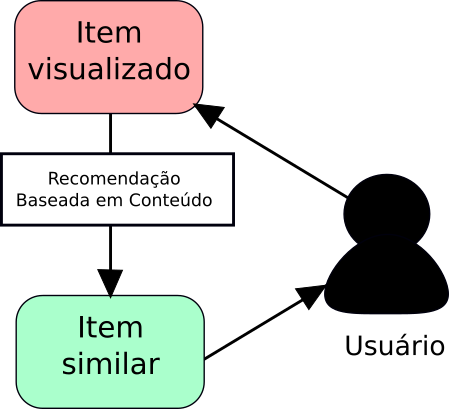
\includegraphics[scale=0.65]{images/recomconteudo.png}
    \label{fig:recomconteudo}
\end{figure}

\subsubsection{Recomendação Híbrida}

A utilização de ambas abordagens (recomendação baseada em conteúdo e filtragem colaborativa) para constituição de um sistema de recomendação é uma técnica utilizada por alguns sistemas de recomendação para aproveitar melhor as características de ambas as abordagens \cite{balabanovic1997fab}.

Nesse contexto, existem algumas formas distintas de combinar técnicas de recomendação, que estão contidas na Tabela \ref{tab:hybrid} \cite{burke2007hybrid}.

\begin{table}[ht]
    \centering
    \ABNTEXchapterfont
    \caption{Descrição dos métodos de hibridação}
    \begin{tabular}{|m{4.0cm}|m{10.0cm}|}
    \hline
        \textbf{Método} & \textbf{Descrição} \\
        \hline
        \hline
        \textbf{Ponderado} & Os resultados dos sistemas de recomendação são combinados para produzir uma única recomendação. \\
        \hline
        \textbf{Alternante} & O sistema alterna entre os diferentes recomendadores de acordo com a situação. \\
        \hline
        \textbf{Combinação de características} &  Características de diferentes fontes de recomendação são colocadas juntos em um único algoritmo de recomendação. \\
        \hline
        \textbf{Mistura} & Recomendações de vários recomendadores são apresentadas ao mesmo tempo. \\
        \hline
        \textbf{Cascata} & Um recomendador refina as recomendações apresentadas pelo outro. \\
        \hline
        \textbf{Acréscimo de característica} & A saída de uma técnica é utilizada como entrada de característica para outra técnica. \\
        \hline
        \textbf{Meta-nível} & O modelo aprendido por um recomendador é utilizado como entrada para outro recomendador. \\
        \hline
    \end{tabular}
    \label{tab:hybrid}
\end{table}

\subsection{Aplicações}

O uso de tecnologias de recomendação é bastante presente em plataformas de computação em nuvem, e mostram-se bastante eficazes na arte de influenciar o usuário final a tomar uma decisão baseada naquilo que lhe é sugerido \cite{shani2011evaluating}. O uso de um sistema de recomendação varia de acordo com o modelo de negócio utilizados e sua plataforma necessária para funcionamento. As pesquisas em sistemas de recomendação são feitas com ênfase principalmente nas aplicações comerciais, já que, sem desemerecer suas contribuições teóricas, há uma preocupação em melhorar sua praticidade comercial \cite{ricci2011introduction}.

Sistemas como esse também são amplamente utilizados na área do comércio virtual, mais conhecido como \emph{e-commerce} \cite{sarwar2002recommender}, fazendo a sugestão de produtos e anúncios para usuários que demonstram interesses em determinadas categorias pela internet. De uma forma geral, podemos descrever o uso prático de sistemas de recomendação nas seguintes áreas \cite{ricci2011introduction}:

\begin{itemize}
    \item \textbf{Entretenimento:} recomendações de filmes, séries, desenhos, músicas, jogos.
    \item \textbf{Conteúdo:} jornais personalizados, recomendação de documentos, livros, páginas \emph{web}, aplicações em aprendizado a distância, fitros de \emph{e-mails}.
    \item \textbf{E-commerce:} recomendação para consumidores para comprar produtos como livros, câmeras, computadores etc.
    \item \textbf{Serviços:} recomendação de serviços de viagens, recomendação de experts para consultas, recomendação de casas para alugar, ou serviços que combinem duas pessoas, como um aplicativo de encontros, ou até mesmo sugestão de oponentes em algum jogo.
\end{itemize}

Os sistemas de recomendação também ajudam a melhorar as vendas de três formas \cite{schafer2001commerce}:

\begin{itemize}
    \item \textbf{Convertendo visitantes em consumidores:} Visitantes de seu \emph{web site} frequentemente acessam o serviço sem intenção de comprar nada. Os sistemas ajudam os consumidores a encontrar itens que potencialmente eles possam se interessar e comprar.
    \item \textbf{Aumentar a venda cruzada:} Sistemas de recomendação podem ajudar a aumentar a venda cruzada através da sugestão de itens adicionais para que o consumidor possa comprar. Nesse caso, o serviço pode recomendar produtos adicionais durante o processo de pagamento, baseado nos produtos que já estão no carrinho de compras.
    \item \textbf{Construir fidelidade:} A fidelidade de clientes é muito importante na área de comércio. Com um bom sistema de recomendação que atenda às necessidades do seu usuário, o cliente saberá que ao visitar aquele determinado \emph{web site} ele terá uma experiência de compra personalizada, e sempre voltará a comprar no mesmo serviço. Isso não só ajuda o próprio sistema de recomendação a refinar seu conhecimento sobre o cliente, como também traz lucro para a companhia.
\end{itemize}

Neste contexto, serão abordados neste trabalho, de forma prática, o uso de sistemas de recomendações em redes sociais, \emph{e-commerce}, em serviços diferentes e até mesmo em estudos e pesquisas de áreas como medicina e biologia.

\subsubsection{Redes sociais}

Sistemas de recomendação são onipresentes nas redes sociais, e tornaram-se importantes para formar conexões entre usuários, vender produtos e descobrir novos conteúdos nessas mídias \cite{burke2007hybrid}. Eles se tornaram partes importantes de \emph{web sites} como YouTube, Facebook, LinkedIn, Twitter e Instagram, por exemplo.

Um bom exemplo do uso de sistemas de recomendação nesse âmbito é o algoritmo de recomendação de vídeos utilizado pelo YouTube. Um estudo realizado em 2010 \cite{zhou2010impact}, mostra uma correlação entre o sistema de recomendação de vídeos do YouTube e as visualizações de cada vídeo afetado, indicando que a maioria das visualizações desses vídeos recomendados pelo \emph{web site} advinham da própria recomendação.

No caso do Facebook, a maior parte dos sistemas de recomendação são baseados em Filtragem Colaborativa \cite{shapira2013facebook}, em que ele usa dados coletados dos usuários que têm interesses e postagens em comum para sugerir conteúdos que também coincidam com tais interesses. O Facebook, assim como LinkedIn, Twitter e Instagram, também possuem sistemas de recomendações de pessoas que possam fazer parte do círculo social do indivíduo, uma abordagem também baseada na Filtragem Colaborativa, que tem se mostrado bastante poder nessas situações por ser capaz de reunir gostos similares dos usuários e conseguir calcular níveis de confiança em amizades \cite{chen2010social}.

\subsubsection{\emph{E-commerce}}

Uma das maiores áreas que utilizam sistemas de recomendação é o âmbito do \emph{e-commerce}, conhecido também como comércio virtual \cite{schafer1999recommender}. Neste, destacam-se no mercado brasileiro grandes nomes do varejo e vendas em geral como Walmart, Carrefour, Saraiva, Casas Bahia, Pontofrio etc. e outras empresas focadas exclusivamente no comércio virtual como Amazon, Mercado Livre, KaBuM, dentre outras tantas que surgiram nos últimos anos.

Sites como Amazon.com apresentam sistemas de recomendação que mostram produtos similares a itens visualizados recentemente, sistemas com recomendações personalizadas para usuários, ofertas mais baratas, e também um sistema que mostra os itens mais comprados pelos usuários (ofertas em alta ou mais vendidos) \cite{schafer2001commerce}. Tal prática também é seguida por diversos outros serviços de \emph{e-commerce} disponíveis.

\subsubsection{Serviços}

Como visto anteriormente, serviços como Netflix focam bastante em sistemas de recomendação para melhorar a experiência do usuário com seus serviços. Utilizando tal serviço como exemplo, pode-se identificar diversos exemplos do uso de sistemas de recomendação na sua página inicial \cite{gomez2016netflix}, como ilustram as Figuras \ref{fig:netflixconteudo} e \ref{fig:netflix}.

\begin{figure}[H]
    \centering
    \caption{Exemplo de recomendação por conteúdo assistido anteriormente e filmes relevantes}
    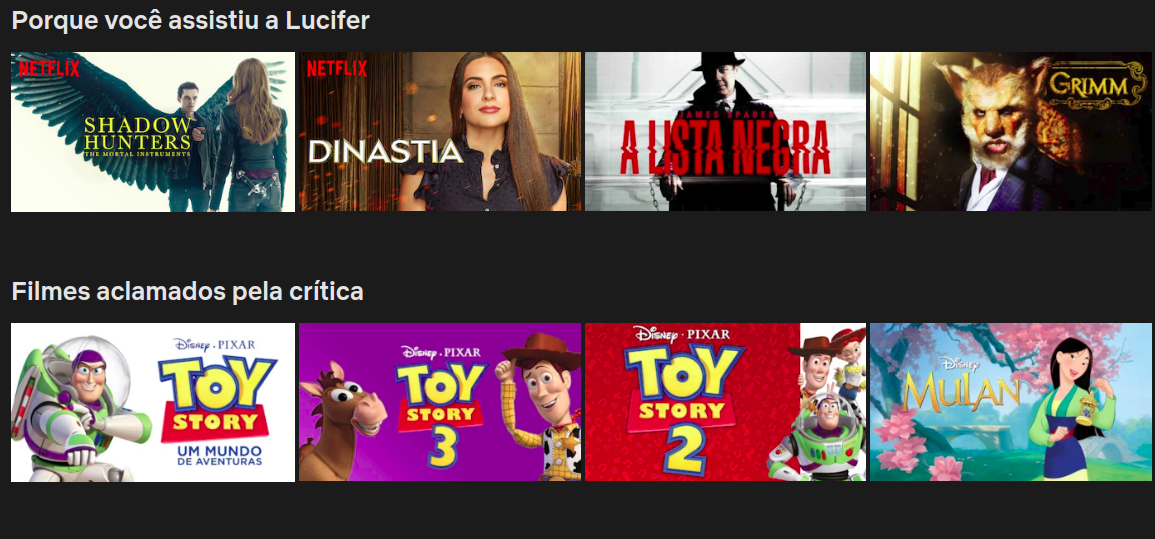
\includegraphics[scale=1.5]{images/netflix.png}
    \label{fig:netflixconteudo}
\end{figure}

Como pode-se observar na Figura \ref{fig:netflixconteudo}, os conteúdos sugeridos baseiam-se no conteúdo de itens previamente assistidos e na coluna seguinte mostra filmes bem avaliados de modo geral, que se encaixam no perfil do usuário em questão.

\begin{figure}[H]
    \centering
    \caption{Exemplo de recomendação personalizada}
    
\includegraphics[scale=1.5]{images/netflixcontent.png}
    \label{fig:netflix}
\end{figure}

Já na Figura \ref{fig:netflix}, os conteúdos sugeridos baseiam-se no perfil do usuário construído pelo sistema de recomendação, e também associa o conteúdo a perfis similares, o que leva a uma série de sugestões personalizadas ao usuário final. Tal prática exemplificada pelo serviço Netflix também é replicada por muitos outros serviços da categoria, como Amazon Prime, Hulu, entre outros.

\section{Trabalhos relacionados}

Tratando-se de computação em nuvem, há diversos trabalhos e aplicações publicados que podem ser mencionados. Os serviços do Microsoft Azure, que fazem parte dessa área, têm sido utilizados em diversas pesquisas distintas, como pesquisa em geoprocessamento \cite{gong2010geoprocessing}, predição de estruturas de proteínas em 3D \cite{mrozek2015scaling} e utilização de aprendizado de máquina em pesquisa de radiologia \cite{kohli2017implementing}.

Também pode-se mencionar trabalhos utilizando serviços da Amazon, como os trabalhos na área da Biomedicina utilizando computação em nuvem \cite{fusaro2011biomedical}, experimento com sequenciamento genômico chamado \textbf{Globus Genomics} \cite{madduri2014experiences} e análise de performance de computação de alto desempenho \cite{jackson2010performance}. Tais artigos demonstram o potencial crescente de plataformas de computação em nuvem, e demonstram que tais ambientes podem ser utilizados com sucesso em pesquisas importantes, nas quais a obtenção de ferramentas computacionais poderosas próprias é bastante dificultada ou quase impossível.

No âmbito de tolerância a falhas em computação em nuvem, este trabalho está associado ao projeto realizado por \citeauthor{andrade2019taxonomia} (\citeyear{andrade2019taxonomia}), que realizou uma revisão sistemática da literatura e implementou um sistema de classificação de técnicas de tolerância a falhas.

Na área de sistemas de recomendação, \citeauthor{adomavicius2005toward} (\citeyear{adomavicius2005toward}) realizou um \emph{survey} sobre o estado da arte desse tipo de tecnologia, levando em consideração trabalhos de \citeauthor{resnick1994grouplens} (\citeyear{resnick1994grouplens}), \citeauthor{hill1995recommending} (\citeyear{hill1995recommending}) e \citeauthor{balabanovic1997fab}, que implementaram seus sistemas de recomendação e introduziram diferentes abordagens para execução.

\section{Considerações finais}

Serviços de computação em nuvem são praticamente onipresentes na vida de usuários de sistemas computacionais nos dias modernos. Pesquisadores se esforçam diariamente para manter os sistemas operantes e livre de quaisquer tipos de falhas que possam vir a comprometer seu funcionamento em tempo de execução. Como pôde ser visto, o número de técnicas de tolerância a falhas é bastante elevado e pode causar confusão em administradores de sistemas.

Nesse âmbito pode-se observar uma lacuna em que se encaixa um sistema de recomendação para as técnicas de tolerância a falhas mais comuns, já que não foi possível encontrar na literatura quaisquer tentativas que caminhassem nessa direção.

\chapter{Projeto}\label{cap_projeto}

O projeto em questão consiste na implementação de um sistema de recomendação para técnicas de tolerância a falhas utilizando os dados coletados em um trabalho realizado por \citeauthor{andrade2019taxonomia} (\citeyear{andrade2019taxonomia}). Nesse trabalho foi desenvolvido um aplicativo com as informações sobre as técnicas de tolerância dispostas em forma de tabelas estáticas.

Levando isso em consideração, este projeto visa aprimorar tal conceito, implementando uma forma de armazenar os dados contidos nessas tabelas em um arquivo de troca de dados, para que os usuários consigam interagir com esses elementos, criando um sistema de recomendação em cima desses dados e permitindo a busca por caracteres relevantes. Dessa forma, a ferramenta desenvolvida se torna ideal para a busca de técnicas de tolerância a falhas, de uma forma intuitiva e facilitada para o usuário final.

\section{Motivação}

O intuito deste trabalho é facilitar a pesquisa de técnicas de tolerância a falhas por meio de uma ferramenta gráfica intuitiva, com recomendação de técnicas e com a possibilidade de pesquisa. Para isso, utilizamos os dados coletados no trabalho citado anteriormente, alimentando este projeto com informações sobre as diferentes 52 técnicas de tolerância a falhas, permitindo sua pesquisa e recomendação na ferramenta.

Assim, o projeto final deve apresentar uma interface gráfica básica e um sistema de recomendação, que poderá filtrar por tipo de falha, podendo ser acessado e aprimorado pelo usuário, por meio da avaliação das técnicas apresentadas.

\section{Metodologia}

Neste projeto será utilizado o \emph{framework} Ionic para implementação do projeto e sua interface gráfica, um sistema de recomendação básico escrito em Python, utilizando biblioteca oferecidas pela linguagem de programação e o \emph{framework} Flask para fazer a comunicação entre os sistemas.

\subsection{Descrição do Sistema}

O sistema proposto neste trabalho trata-se de um protótipo de uma ferramenta com sistema de recomendação que pode ser utilizado e expandido para uso posterior ou para quaisquer outros propósitos. Nesta ferramenta, os itens a serem recomendados são as técnicas de tolerância a falhas, e o usuário poderá filtrar as técnicas por tipos de falhas, ou então poderá pesquisá-las por meio de uma barra de busca. O intuito dessa ferramenta é auxiliar o trabalho de administradores de sistemas que demandam tolerância a falhas, tornando mais simples o trabalho de pesquisa e comparação de técnicas de tolerância a falhas, permitindo também que o usuário avalie a técnica disponível e consiga aperfeiçoar o sistema para outros usuários.

Na figura \ref{fig:mockup} está representado um projeto da tela inicial do sistema e seus principais componentes: a pesquisa, a filtragem pelas falhas (\emph{tags}) e os \emph{cards} com as informações das técnicas de tolerância recomendadas.

\begin{figure}[H]
    \centering
    \caption{Planejamento inicial de interface da ferramenta}
    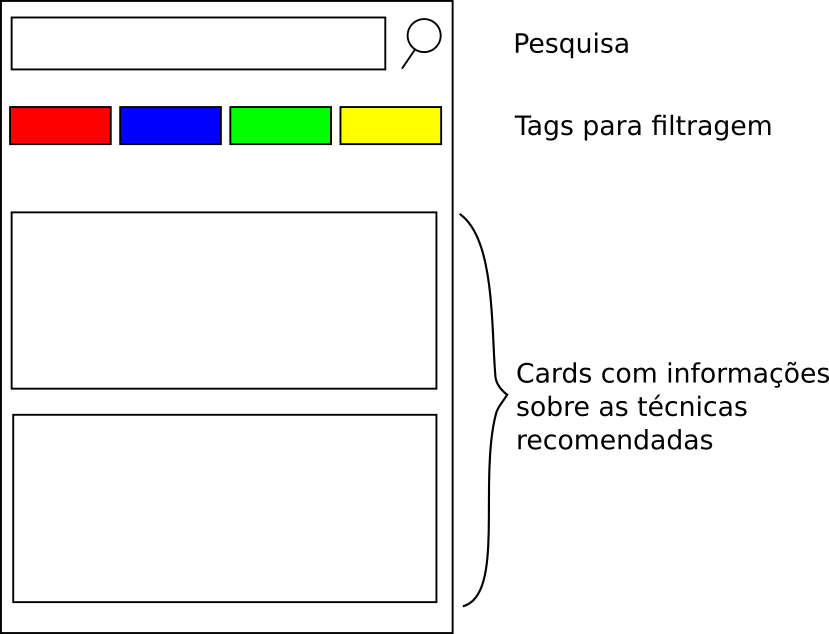
\includegraphics[width=12.0cm,height=8.0cm]{images/mockup.png}
    \label{fig:mockup}
    \textual
\end{figure}

\subsection{Desafios}

Uma grande parte do conteúdo disponível sobre sistemas de recomendação está voltado para itens mais comuns no cotidiano, como serviços de \emph{e-commerce}, recomendação de filmes e itens, recomendação de amizades ou conexões prováveis, dentre tantas outras aplicações que estão distantes das formas com que o sistema é aplicado neste trabalho. Além disso, existem inúmeras limitações para sistemas de recomendação com poucos dados, como é o caso deste trabalho, em que os dados coletados e disponíveis não estão calibrados suficientemente por uma enorme gama de usuários que utilizam o serviço.

Por conta desses detalhes o trabalho teve de ser adaptado e cuidadosamente trabalhado para evitar que essas limitações viessem a atrapalhar as recomendações resultantes dos itens registrados. As adaptações feitas estão descritas na seção \ref{sec_imp}, bem como alguns detalhes sobre os algoritmos empregados.

\subsection{Implementação}\label{sec_imp}

O início da implementação do projeto consiste em transformar os dados disponíveis sobre as técnicas de tolerância a falhas em dados que possam ser trabalhados pela aplicação, utilizando tags relevantes e conteúdos que possam ser armazenados em um banco de dados ou em um arquivo de troca de dados, como por exemplo arquivos no formato JSON (JavaScript Object Notation) ou CSV (Comma Separated Values).

Neste projeto, foi escolhido o armazenamento de dados utilizando arquivos JSON e CSV, pela simplicidade oferecida pelos arquivos e pela forma rápida de responsividade desses arquivos utilizando as linguagens Python e JavaScript.

\subsubsection{Coleta de dados}\label{sec_coleta}

Os dados referentes às técnicas de tolerância a falhas foram coletados manualmente em um arquivo de extensão ``.txt'', utilizando as tabelas desenvolvidas no trabalho de \citeauthor{andrade2019taxonomia} (\citeyear{andrade2019taxonomia}), e mais tarde foi utilizado um script desenvolvido em Python pelo autor para adequá-los ao formato JSON.

Cada uma das tabelas descritas no documento foi cuidadosamente analisada, adicionando os dados relevantes para tornar tais tabelas mais compatíveis com um modelo de sistema de recomendação, colocando itens como classificação de usuários. No total, foram identificadas 52 técnicas de tolerância a falhas, divididas em 4 tipos de falhas principais: falhas relacionadas a dados, a processos, a virtualização e a comunicação.

As técnicas selecionadas estão listadas a seguir \cite{andrade2019taxonomia}:

\begin{multicols}{2}
\begin{itemize}
    \item[--] InterGrid Gateway (IGG)
    \item[--] HySARC
    \item[--] SkyCDS
    \item[--] DARGOS
    \item[--] Protótipo para tratamento automático de anomalias
    \item[--] Tahoe-LAFS
    \item[--] SwiftER
    \item[--] Sistema de armazenamento privado multicamadas
    \item[--] Gluster File System (GFS)
    \item[--] Algoritmo híbrido baseado em MapReduce
    \item[--] Morpho
    \item[--] Dynamic Cost-Aware Re-Replication and Re-balancing Strategy (DCR2S)
    \item[--] Fuzzy Inference based Reliable Replica Replacement (FIR3)
    \item[--] Medical Image File Accessing System (MIFAS)
    \item[--] Sistema baseado no princípio 80/20
    \item[--] Middleware de nuvem para garantir desempenho e alta disponibilidade de aplicativos soft em tempo real
    \item[--] mOSAIC
    \item[--] Pilot-Data
    \item[--] ONHelp
    \item[--] Sistema de resgate de spot inesperados usando instâncias de spot heterogêneos e excesso de provisão
    \item[--] Symbiotic Virtualization (SymVirt)
    \item[--] Mantis
    \item[--] Fault-Tolerant Stateful Firewall (FT-FW)
    \item[--] Sistema de controle de acesso avançado
    \item[--] Protótipo para Extração sistemática dos estados de rede
    \item[--] pFTree-Ext e pFTree-Wt
    \item[--] Auto healing service framework
    \item[--] Mayflies
    \item[--] TOPSIS
    \item[--] Group-U
    \item[--] Dering Over Shared Memory (DORADO)
    \item[--] COSCAnet-FT
    \item[--] Cloud Inter-operation Toolkit(CIT)
    \item[--] OpenADN
    \item[--] SprintNet
    \item[--] Future Automation System Architecture (FASA)
    \item[--] Fault Tolerance Manager (FTM)
    \item[--] Fault-tolerance in federated Clouds (FT-FC)
    \item[--] Promethee Scheduler
    \item[--] Proposta de arquitetura de cluster virtual tolerante a falhas
    \item[--] Cloud-Agnostic Checkpointing Service (CACS)
    \item[--] Unibus
    \item[--] Availability Knob
    \item[--] Protótimo para Sistema de Migração de VM
    \item[--] Fault-Tolerant Elastic Scheduling Algortihm for Workflow (FTESW)
    \item[--] Sistema de detecção e mitigação de falhas
    \item[--] Algoritmo de tolerância a falhas energéticas para computação de alto desempenho
    \item[--] Zurmo Native
    \item[--] Proactive Fault Tolerance Mechanism for Data Center Network
    \item[--] Replicação de VM para melhorar a capacidade de sobrevivência de aplicativos de missão crítica
    \item[--] HAStack
    \item[--] FTStack
\end{itemize}
\end{multicols}

Cada uma das características de cada técnica foi extraída e compilada de forma adequada no arquivo de dados JSON correspondente. Dessa forma, cada uma das técnicas cadastradas no sistema possui um conjunto único de características e permite que o usuário possa visualizá-las para poder fazer a comparação e descobrir suas vantagens e desvantagens. As características essenciais são: Nome, Técnicas utilizadas, Gestor de Nuvem, Modelo de implementação, Problema que visa solucionar, Tipo de falha tratada, Vantagens e, por fim, Desvantagens.

Um aspecto importante para um sistema de recomendação é a avaliação de usuários sobre as técnicas em questão. É importante que haja uma relação direta entre usuários e as técnicas para que o sistema de recomendação produza resultados precisos e refinados. Entretanto, tais sistemas geralmente trabalham com grandes quantidades de dados, e quando não há uma grande coleção de informações para trabalhar, as recomendações feitas são bastante imprecisas.

Um dos maiores problemas de sistemas de filtragem colaborativa é o problema \emph{cold-start}, que descreve justamente o que foi mencionado anteriormente: novos itens ou novos usuários não possuem dados suficientes para que se possa fazer uma recomendação baseada em seu perfil ou em características descritas \cite{lika2014facing,lam2008addressing}.

Para que se possa validar os testes do sistema, deve-se então possuir uma ampla base de usuários e dados que validem as recomendações feitas. No entanto, como este trabalho possui um número bastante limitado de usuários e sequer se trata de um produto de larga escala, realizar essa validação pode parecer impossível.

Dessa forma, para contornar este problema inicial foi feita a geração de dados aleatórios seguindo uma distribuição normal para diferentes quantidades de usuários, e também para servir de base para o sistema inicial. Assim, é possível produzir recomendações básicas para usuários do sistema e evitar o problema inicial para as propostas deste trabalho. Na seção \ref{sec:geracao} será discutido como tal método foi implementado.

\subsubsection{Geração de dados}\label{sec:geracao}

Os dados utilizados para os testes de validação do sistema de recomendação foram gerados de forma automática, utilizando um \emph{script} em Python escrito pelo próprio autor que gera um arquivo em CSV com os seguintes componentes:

\begin{itemize}
    \item Identificador do Usuário (UID)
    \item Identificador da Técnica (IID)
    \item Avaliação Consolidada (Rating)
\end{itemize}

O \emph{script} em questão gera um identificador aleatório para o usuário e também gera um valor no intervalo de 0 a 51, correspondendo às 52 técnicas propostas, e assinala uma avaliação que segue uma distribuição gaussiana com os parâmetros $\mu = 3$ e $\sigma = 1$, obtendo resultados mais próximos de uma avaliação real em termos estatísticos. Para as finalidades deste trabalho, os valores de avaliação gerados foram arredondados utilizando uma função piso, evitando assim qualquer tipo de conflito durante os cálculos de avaliações.

Além disso, o \emph{script} também checa para ver se a tupla usuário e técnica já foi registrada anteriormente, evitando registrar duas avaliações distintas para o mesmo usuário, o que também apresentaria um problema para o sistema de recomendação.

Com esses dados é possível fazer com que o sistema de recomendação faça sugestões com melhor precisão, evitando o problema descrito anteriormente. Assim, recebendo um parâmetro $x$ e um determinado número de usuários (\textbf{nuser}), o \emph{script} é capaz de gerar o produto desses dois parâmetros como o total de avaliações possíveis.

Por exemplo, se for estabelecido: $x = 10$ e $\text{nuser}=5$, então teremos um total de 50 avaliações nos arquivos de dados.

Com isso, foram gerados seis diferentes arquivos de extensão CSV para os testes dos dados, com o seguinte nome: \textbf{userdata\_x\_nuser.csv}. Escolhendo o parâmetro $x = 5$ e $x=10$ de maneira arbitrária, com um número de usuários crescente, partindo de 10 usuários até 1000, os seguintes arquivos foram gerados:

\begin{itemize}
    \item userdata\_5\_10.csv
    \item userdata\_5\_100.csv
    \item userdata\_5\_1000.csv
    \item userdata\_10\_10.csv
    \item userdata\_10\_100.csv
    \item userdata\_10\_1000.csv
\end{itemize}

Tais parâmetros foram escolhidos para simplificar a disposição dos testes neste documento.

Todos os arquivos mencionados, incluindo o código fonte do \emph{script} mencionado estão disponíveis na página do projeto no GitHub.

\subsubsection{Armazenamento de dados}

Os dados coletados e gerados são armazenados em formatos de arquivos simples JSON e CSV, como mencionado anteriormente. A simplicidade e rapidez que o trabalho com essas extensões de arquivos oferece torna desnecessário o uso de algum sistema de gerenciamento de banco de dados mais robusto, pelo menos para os propósitos deste trabalho.

\subsubsection{Sistema de Recomendação}

O sistema de recomendação implementado segue o modelo de filtragem colaborativa, por ser o modelo mais amplamente utilizado na indústria, o mais robusto e confiável nesse quesito.

A implementação do sistema de recomendação referente teve de ser bastante cautelosa e profundamente estudada. Existem inúmeros algoritmos que compõem sistemas de recomendação de diversos tipos, e, neste projeto, construir um sistema de recomendação que seja capaz de validar resultados e que seja flexível o suficiente era o maior objetivo. A implementação de cada um desses algoritmos de forma eficiente e otimizada tornou-se inviável para a proposta deste trabalho, e por esse motivo optou-se por uma biblioteca especializada para esse tipo de aplicação.

A linguagem Python possui grandes aplicações na área de inteligência artificial em geral, e as formas de lidar com ciência de dados são bastante numerosas. Não surpreendentemente, existem diversas bibliotecas que possibilitam a implementação de sistemas de recomendação usando a linguagem.

Dessa forma, para tornar mais prático o trabalho de implementação de diversos tipos de sistemas de recomendação, e ser capaz de realizar testes de validação das previsões desses sistemas, será utilizada a ferramenta \textbf{Surprise} \cite{Surprise}, uma biblioteca em Python que facilita a implementação e validação de sistemas de recomendação de filtragem colaborativa. Tal ferramenta é composta por algoritmos matemáticos como a decomposição em valores singulares, máxima verossimilhança, fatorização de matrizes, k-NN, entre outras abordagens matemáticas e estatísticas que são aplicadas nesse âmbito.

Além disso, a ferramenta tem funções para lidar com conjuntos de dados (\emph{datasets}) e possibilita o treinamento dos algoritmos mencionados, para obtenção de melhores resultados.

\subsubsection{Interface gráfica}

A interface gráfica da ferramenta foi implementada usando o \emph{framework} Ionic com a plataforma Angular. Tal interface conecta-se ao sistema desenvolvido em Python por meio de um intermediário, o Flask, um \emph{framework web} escrito em Python.

Os \emph{cards} de recomendação com as informações das técnicas utilizam os dados processados pelo sistema de recomendação e são mostrados na forma de lista pelo Ionic, com as informações básicas dispostas. O usuário, a partir da interface, pode clicar nas respectivas técnicas para obter informações detalhadas sobre elas. Além disso, a interface gráficas possui uma barra de pesquisa que permite filtragem por \emph{tags} diversas, que serão descritas na seção \ref{sec_interface}.

\section{Considerações finais}

Neste capítulo foram apresentados todos os procedimentos relevantes para a implementação do projeto, bem como os desafios e funcionalidades planejados. No capítulo a seguir, serão apresentados os testes realizados utilizando os sistemas implementados, bem como apresentações das funcionalidades da ferramenta em si, mostrando seu potencial para os fins desejados.

\chapter{Testes e Resultados}\label{cap_testes}

Neste capítulo serão apresentados os testes e resultados obtidos utilizando o sistema implementado. De forma geral, serão apresentadas algumas análises dos dados processados, formas de validação dessa análise, e por fim uma visão geral do funcionamento do sistema como um todo.

\section{Validação e Previsões}

Os dados gerados são bastante extensos para uma análise bastante detalhada, pois existem muitas informações a serem consideradas e analisadas. Sabendo disso, podemos utilizar os métodos de validação cruzada disponíveis na biblioteca Surprise para avaliar a precisão das previsões feitas pelo algoritmo de recomendação utilizado.

Nos métodos de validação cruzada serão utilizadas duas formas de medida para determinar tal precisão: o Erro Médio Absoluto, ou \emph{Mean Absolute Error} (MAE), e a Raiz do Erro Quadrático Médio, ou \emph{Root Mean Squared Error} (RMSE).

De forma simplificada, ambas as medidas podem ser utilizadas para a validação de modelos preditivos, sendo bastante utilizadas em aplicações de aprendizado de máquina, modelos de regressão e simulações computacionais. Elas são utilizadas nas chamadas validações cruzadas, que consistem em dividir o conjunto de dados em K conjuntos menores de treino e testes, de forma independente, para que seus resultados sejam comparados e que assim se possa determinar a proximidade dos resultados obtidos na previsão desses conjuntos menores.

As medidas de erro são aplicadas em cada um dos conjuntos de validação cruzada, e quanto mais próximo de zero, mais precisa é a previsão obtida.

\subsection{Primeiro teste}

Neste primeiro teste serão aplicados os algoritmos de validação cruzada para os arquivos que receberam parâmetros $x=5$, ou seja, os arquivos com um número relativamente baixo de dados disponíveis. Assim pode-se estabelecer uma comparação entre os resultados obtidos com poucos dados e os resultados obtidos com muitos dados.

Primeiramente é necessário escolher um algoritmo para o treinamento dos dados e assim poder realizar as previsões. Neste primeiro teste será utilizado o algoritmo de Decomposição em valores singulares, e o código para executar todo esse treinamento e validação é o seguinte:

\begin{minted}{python}
def get_predictions(dataset):
    reader = Reader(line_format='user item rating', sep=',', rating_scale=(1, 5))
    data = Dataset.load_from_file(dataset, reader=reader)
    trainset = data.build_full_trainset()
    algo = SVD()
    algo.fit(trainset)

    testset = trainset.build_anti_testset()
    predictions = algo.test(testset)

    cross_validate(algo, data, measures=['RMSE', 'MAE'], cv=5, verbose=True)
    
get_predictions('userdata_5_10.csv')
get_predictions('userdata_5_100.csv')
get_predictions('userdata_5_1000.csv')
\end{minted}

Deve-se notar que a cada execução, os dados obtidos dos algoritmos variam, assim como suas previsões realizadas, e isso pode prejudicar a reprodutibilidade dos resultados. O motivo desta mudança é que a cada execução a biblioteca Surprise gera um número aleatório para a validação cruzada e predição de algoritmos.

Para resolver este problema, o \emph{script} utilizado utiliza um valor de semente $seed=0$ para a biblioteca \emph{random} do Python. Todos os testes executados neste documento utilizarão o mesmo valor de semente, para que esses resultados sejam reprodutíveis posteriormente. O seguinte código deve ser incluído no código fonte a ser executado:

\begin{minted}{python}

import random
import numpy as np

my_seed = 0
random.seed(my_seed)
np.random.seed(my_seed)
\end{minted}

Com os parâmetros estabelecidos, os resultados obtidos na validação cruzada de cada um dos arquivos gerados estão descritos nas tabelas \ref{tab:teste1}, \ref{tab:teste2} e \ref{tab:teste3}.

\begin{table}[ht]
    \centering
    \ABNTEXchapterfont
    \caption{Teste com o arquivo userdata\_5\_10.csv}
    \begin{tabular}{|m{1.5cm}|m{1.5cm}|m{1.5cm}|m{1.5cm}|m{1.5cm}|m{1.5cm}|m{1.5cm}|}
    \hline
        \textbf{Medida}& \textbf{Fold 1} & \textbf{Fold 2} & \textbf{Fold 3} & \textbf{Fold 4}& \textbf{Fold 5} & \textbf{Média}\\
        \hline
        \hline
        \textbf{RMSE} & 1.0986 & 0.8522 & 1.0072 & 1.0630 & 1.0661 & 1.0174  \\ 
        \hline
        \textbf{MAE} & 0.9509 & 0.6995 & 0.8610 & 0.8912 & 0.9178 & 0.8641 \\
        \hline
    \end{tabular}
    \label{tab:teste1}
\end{table}

\begin{table}[ht]
    \centering
    \ABNTEXchapterfont
    \caption{Teste com o arquivo userdata\_5\_100.csv}
    \begin{tabular}{|m{1.5cm}|m{1.5cm}|m{1.5cm}|m{1.5cm}|m{1.5cm}|m{1.5cm}|m{1.5cm}|}
    \hline
        \textbf{Medida}& \textbf{Fold 1} & \textbf{Fold 2} & \textbf{Fold 3} & \textbf{Fold 4}& \textbf{Fold 5} & \textbf{Média}\\
        \hline
        \hline
        \textbf{RMSE} & 1.1350 & 1.0167 & 0.9913 & 1.0644 & 0.9738 & 1.0362 \\ 
        \hline
        \textbf{MAE} & 0.9513 & 0.8564 & 0.8235 & 0.8928 & 0.8213 & 0.8690\\
        \hline
    \end{tabular}
    \label{tab:teste2}
\end{table}

\begin{table}[ht]
    \centering
    \ABNTEXchapterfont
    \caption{Teste com o arquivo userdata\_5\_1000.csv}
    \begin{tabular}{|m{1.5cm}|m{1.5cm}|m{1.5cm}|m{1.5cm}|m{1.5cm}|m{1.5cm}|m{1.5cm}|}
    \hline
        \textbf{Medida}& \textbf{Fold 1} & \textbf{Fold 2} & \textbf{Fold 3} & \textbf{Fold 4}& \textbf{Fold 5} & \textbf{Média}\\
        \hline
        \hline
        \textbf{RMSE} & 1.0064 & 1.0083 & 0.9964 & 0.9933 & 1.0135 & 1.0036 \\ 
        \hline
        \textbf{MAE} & 0.8403 & 0.8444 & 0.8216 & 0.8251 & 0.8393 & 0.8341 \\
        \hline
    \end{tabular}
    \label{tab:teste3}
\end{table}

Pode-se observar das tabelas que os valores obtidos estão bastante próximos de 1, o que nos diz que a margem de erro das previsões feitas é baixa, mas que ainda assim não é precisa o suficiente. Isso se deve talvez pelo baixo número de avaliações disponíveis nos arquivos.

\subsection{Segundo teste}

De maneira similar ao teste anterior, os testes desta seção serão executados nos arquivos gerados que receberam parâmetro $x=10$, tratando-se então de um conjunto de dados relativamente maior que o anterior. As alterações no código descritas anteriormente apenas limitaram-se apenas à mudança dos arquivos de dados gerados.

Os resultados obtidos desses novos testes encontram-se nas tabelas \ref{tab:teste4}, \ref{tab:teste5} e \ref{tab:teste6}.

\begin{table}[ht]
    \centering
    \ABNTEXchapterfont
    \caption{Teste com o arquivo userdata\_10\_10.csv}
    \begin{tabular}{|m{1.5cm}|m{1.5cm}|m{1.5cm}|m{1.5cm}|m{1.5cm}|m{1.5cm}|m{1.5cm}|}
    \hline
        \textbf{Medida}& \textbf{Fold 1} & \textbf{Fold 2} & \textbf{Fold 3} & \textbf{Fold 4}& \textbf{Fold 5} & \textbf{Média}\\
        \hline
        \hline
        \textbf{RMSE} & 1.2226 & 1.2449 & 1.3538 & 1.0392 & 0.9741 & 1.1669   \\ 
        \hline
        \textbf{MAE} & 1.0095 & 1.0007 & 1.1697 & 0.8224 & 0.7771 & 0.9559 \\
        \hline
    \end{tabular}
    \label{tab:teste4}
\end{table}

\begin{table}[ht]
    \centering
    \ABNTEXchapterfont
    \caption{Teste com o arquivo userdata\_10\_100.csv}
    \begin{tabular}{|m{1.5cm}|m{1.5cm}|m{1.5cm}|m{1.5cm}|m{1.5cm}|m{1.5cm}|m{1.5cm}|}
    \hline
        \textbf{Medida}& \textbf{Fold 1} & \textbf{Fold 2} & \textbf{Fold 3} & \textbf{Fold 4}& \textbf{Fold 5} & \textbf{Média}\\
        \hline
        \hline
        \textbf{RMSE} & 0.9977 & 1.0369 & 1.0416 & 1.0479 & 1.0037 & 1.0256\\ 
        \hline
        \textbf{MAE} & 0.8316 & 0.8675 & 0.8781 & 0.8501 & 0.8234 & 0.8502\\
        \hline
    \end{tabular}
    \label{tab:teste5}
\end{table}

\begin{table}[ht]
    \centering
    \ABNTEXchapterfont
    \caption{Teste com o arquivo userdata\_10\_1000.csv}
    \begin{tabular}{|m{1.5cm}|m{1.5cm}|m{1.5cm}|m{1.5cm}|m{1.5cm}|m{1.5cm}|m{1.5cm}|}
    \hline
        \textbf{Medida}& \textbf{Fold 1} & \textbf{Fold 2} & \textbf{Fold 3} & \textbf{Fold 4}& \textbf{Fold 5} & \textbf{Média}\\
        \hline
        \hline
        \textbf{RMSE} & 1.0190 & 1.0149 & 1.0354 & 0.9931 & 1.0313 & 1.0188 \\ 
        \hline
        \textbf{MAE} & 0.8459 & 0.8404 & 0.8538 & 0.8208 & 0.8527 & 0.8427\\
        \hline
    \end{tabular}
    \label{tab:teste6}
\end{table}

Neste novo caso, os valores ainda estão mais próximos de 1, o que indica uma margem de erro próxima àquela vista nos testes anteriores, mesmo com um volume maior de dados. De forma geral, pode-se notar por esses testes que a distribuição das avaliações tem grande impacto no valor obtido no erro de previsões, e não somente pela quantidade de dados disponíveis.

Ainda assim, os dados gerados não estão tão longe de uma aplicação real, em que a margem de erro também gira em torno de 0,7 a 1,1 na maioria dos casos. Isso significa que o sistema é sim capaz de gerar boas recomendações utilizando o algoritmo descrito, mas também há margem para melhores recomendações.

\subsection{Terceiro teste}

Dessa vez, de forma sucinta, serão apresentados os dados obtidos de todos os arquivos utilizando um algoritmo de previsão diferente, conhecido como Matriz de Fatorização Não-Negativa, ou NMF. Neste caso a única alteração no código foi relacionada ao algoritmo usado foi a mudança do valor de $algo = SVD()$ para $algo = NMF()$, que é a função já implementada do algoritmo na biblioteca. 

Tal algoritmo é bastante utilizado em diversas outras áreas computacionais, como bioinformática, processamento de sinais, aprendizado de máquina e visão computacional, também tendo um papel bastante importante em sistemas de recomendação por filtragem colaborativa \cite{lee2001algorithms}.

As tabelas \ref{tab:teste7}, \ref{tab:teste8}, \ref{tab:teste9}, \ref{tab:teste10}, \ref{tab:teste11} e \ref{tab:teste12} representam os resultados obtidos segundo os parâmetros estabelecidos previamente.

\begin{table}[ht]
    \centering
    \ABNTEXchapterfont
    \caption{Teste com o arquivo userdata\_5\_10.csv usando matriz de fatorização não-negativa}
    \begin{tabular}{|m{1.5cm}|m{1.5cm}|m{1.5cm}|m{1.5cm}|m{1.5cm}|m{1.5cm}|m{1.5cm}|}
    \hline
        \textbf{Medida}& \textbf{Fold 1} & \textbf{Fold 2} & \textbf{Fold 3} & \textbf{Fold 4}& \textbf{Fold 5} & \textbf{Média}\\
        \hline
        \hline
        \textbf{RMSE} & 0.7532 & 0.9825 & 0.9904 & 1.0747 & 0.9760 & 0.9553   \\ 
        \hline
        \textbf{MAE} & 0.6006 & 0.8421 & 0.7783 & 0.8695 & 0.7790 & 0.7739 \\
        \hline
    \end{tabular}
    \label{tab:teste7}
\end{table}

\begin{table}[ht]
    \centering
    \ABNTEXchapterfont
    \caption{Teste com o arquivo userdata\_5\_100.csv usando matriz de fatorização não-negativa}
    \begin{tabular}{|m{1.5cm}|m{1.5cm}|m{1.5cm}|m{1.5cm}|m{1.5cm}|m{1.5cm}|m{1.5cm}|}
    \hline
        \textbf{Medida}& \textbf{Fold 1} & \textbf{Fold 2} & \textbf{Fold 3} & \textbf{Fold 4}& \textbf{Fold 5} & \textbf{Média}\\
        \hline
        \hline
        \textbf{RMSE} & 1.2298 & 1.1795 & 1.2699 & 1.3074 & 1.2851 & 1.2544\\ 
        \hline
        \textbf{MAE} & 1.0099 & 0.9216 & 1.0362 & 1.0335 & 1.0565 & 1.0115\\
        \hline
    \end{tabular}
    \label{tab:teste8}
\end{table}

\begin{table}[ht]
    \centering
    \ABNTEXchapterfont
    \caption{Teste com o arquivo userdata\_5\_1000.csv matriz de fatorização não-negativa}
    \begin{tabular}{|m{1.5cm}|m{1.5cm}|m{1.5cm}|m{1.5cm}|m{1.5cm}|m{1.5cm}|m{1.5cm}|}
    \hline
        \textbf{Medida}& \textbf{Fold 1} & \textbf{Fold 2} & \textbf{Fold 3} & \textbf{Fold 4}& \textbf{Fold 5} & \textbf{Média}\\
        \hline
        \hline
        \textbf{RMSE} & 1.2246 & 1.1870 & 1.2114 & 1.2279 & 1.1568 & 1.2015 \\ 
        \hline
        \textbf{MAE} & 0.9810 & 0.9523 & 0.9764 & 0.9881 & 0.9328 & 0.9661\\
        \hline
    \end{tabular}
    \label{tab:teste9}
\end{table}

\begin{table}[ht]
    \centering
    \ABNTEXchapterfont
    \caption{Teste com o arquivo userdata\_10\_10.csv matriz de fatorização não-negativa}
    \begin{tabular}{|m{1.5cm}|m{1.5cm}|m{1.5cm}|m{1.5cm}|m{1.5cm}|m{1.5cm}|m{1.5cm}|}
    \hline
        \textbf{Medida}& \textbf{Fold 1} & \textbf{Fold 2} & \textbf{Fold 3} & \textbf{Fold 4}& \textbf{Fold 5} & \textbf{Média}\\
        \hline
        \hline
        \textbf{RMSE} & 1.4075 & 1.4194 & 1.3718 & 1.2201 & 1.4750 & 1.3788 \\ 
        \hline
        \textbf{MAE} & 1.0163 & 1.1976 & 1.1508 & 0.9800 & 1.0849 & 1.0859 \\
        \hline
    \end{tabular}
    \label{tab:teste10}
\end{table}

\begin{table}[ht]
    \centering
    \ABNTEXchapterfont
    \caption{Teste com o arquivo userdata\_10\_100.csv matriz de fatorização não-negativa}
    \begin{tabular}{|m{1.5cm}|m{1.5cm}|m{1.5cm}|m{1.5cm}|m{1.5cm}|m{1.5cm}|m{1.5cm}|}
    \hline
        \textbf{Medida}& \textbf{Fold 1} & \textbf{Fold 2} & \textbf{Fold 3} & \textbf{Fold 4}& \textbf{Fold 5} & \textbf{Média}\\
        \hline
        \hline
        \textbf{RMSE} & 1.1635 & 1.1435 & 1.1476 & 1.1072 & 1.2127 & 1.1549 \\ 
        \hline
        \textbf{MAE} & 0.9502 & 0.9151 & 0.9485 & 0.8900 & 0.9915 & 0.9391\\
        \hline
    \end{tabular}
    \label{tab:teste11}
\end{table}

\begin{table}[ht]
    \centering
    \ABNTEXchapterfont
    \caption{Teste com o arquivo userdata\_10\_1000.csv matriz de fatorização não-negativa}
    \begin{tabular}{|m{1.5cm}|m{1.5cm}|m{1.5cm}|m{1.5cm}|m{1.5cm}|m{1.5cm}|m{1.5cm}|}
    \hline
        \textbf{Medida}& \textbf{Fold 1} & \textbf{Fold 2} & \textbf{Fold 3} & \textbf{Fold 4}& \textbf{Fold 5} & \textbf{Média}\\
        \hline
        \hline
        \textbf{RMSE} & 1.1523 & 1.1766 & 1.1920 & 1.1729 & 1.1573 & 1.1702\\ 
        \hline
        \textbf{MAE} & 0.9329 & 0.9496 & 0.9654 & 0.9473 & 0.9321 & 0.9455 \\
        \hline
    \end{tabular}
    \label{tab:teste12}
\end{table}

Os resultados com esse algoritmo exibiram uma margem de erro mais elevada do que o algoritmo anterior, mas ainda assim muito próxima do valor 1. Isso mostra o quanto os dados gerados podem produzir resultados relevantes para um sistema de recomendação.

\section{Interface gráfica e recomendações} \label{sec_interface}

A implementação do sistema de recomendação separa os dados das técnicas de tolerância a falhas de suas avaliações dos usuários, utilizando uma lista de números para oferecer recomendações, sem associar esses números com os dados específicos.

Como exemplo, a seguir estão algumas recomendações feitas pelo sistema para os usuários com identificadores 327, 266 e 481, escolhidos de forma arbitrária, ao utilizar um dos algoritmos descritos anteriormente sobre as condições propostas nas seções anteriores:

\begin{minted}{python}
327 ['38', '51', '14', '32', '34', '33', '44', '36', '0', '21']
266 ['5', '17', '21', '39', '15', '34', '3', '47', '8', '19']
481 ['39', '7', '22', '43', '14', '28', '15', '3', '1', '21']
\end{minted}

Neste caso, cada usuário recebe uma recomendação diferente de 10 técnicas, cada uma com seu identificador próprio (IID), sem estar associada a uma técnica em um banco de dados. Dessa forma torna-se complicado conectar os dados de maneira eficiente, e como o sistema é capaz de calcular recomendações para muitos usuários diferentes, torna-se totalmente inviável apresentar cada caso individualmente neste trabalho.

Utilizando a interface gráfica criada, pode-se testar de forma mais eficiente as recomendações obtidas por diferentes usuários. Esta também é uma forma de validação do uso da interface para os propósitos deste projeto, como uma ferramenta fácil e intuitiva para o usuário final.

\begin{figure}[H]
    \centering
    \caption{Tela inicial da ferramenta}
    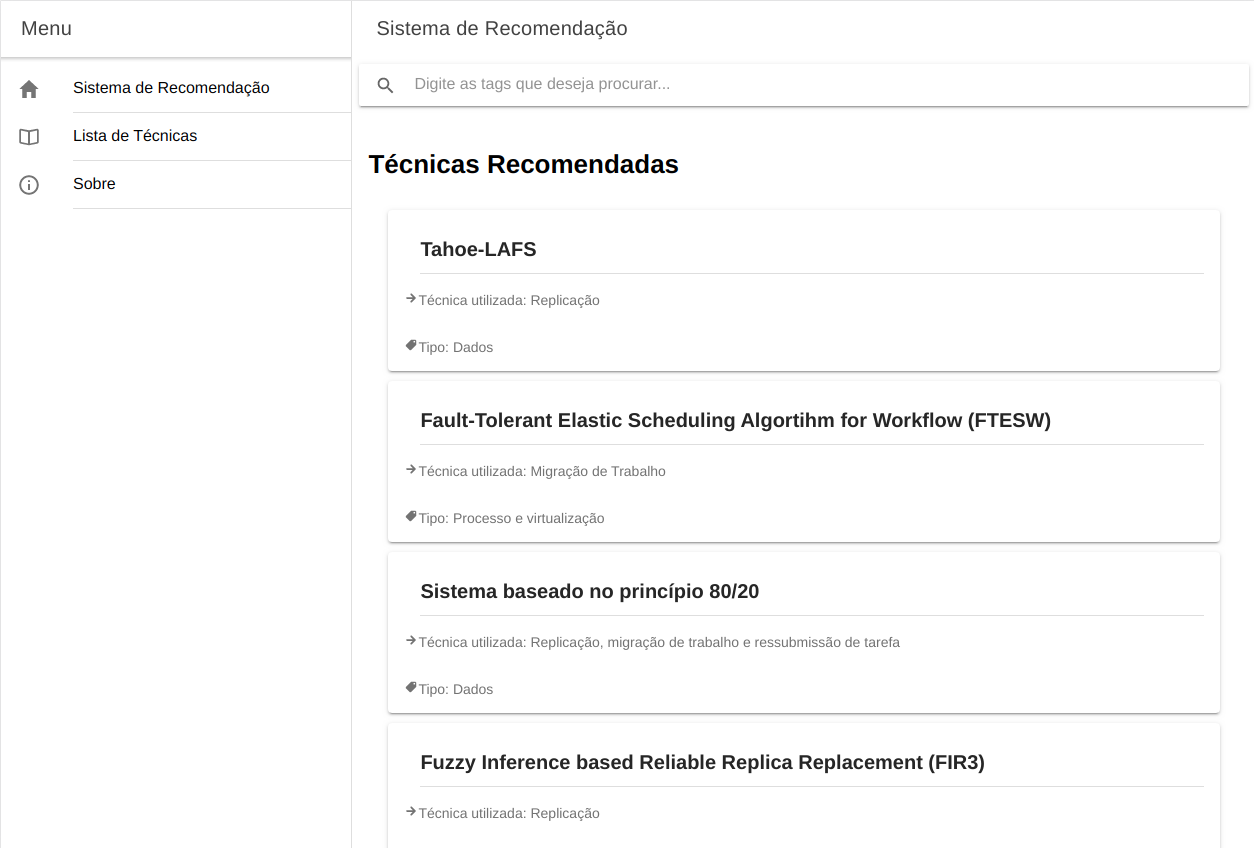
\includegraphics[scale=1.5]{images/sist_recomend.png}
    \label{fig:sisrec_teste}
    \\
\end{figure}

A Figura \ref{fig:sisrec_teste} mostra a interface inicial da ferramenta desenvolvida neste trabalho, mostrando seus aspectos principais de navegação, bem como o sistema de recomendação plenamente funcional. Para intuito de demonstração, foi selecionado o usuário de identificador 8 e as respectivas recomendações calculadas para tal. Pode-se observar que a aplicação apresenta os dados básicos das técnicas 

O sistema de recomendação é acessado pelo \emph{framework} Ionic através de um \emph{request} HTTP com o identificador do usuário à aplicação Flask, que foi mantida em execução para permitir as recomendações. A aplicação Flask executa a cada requisição um novo cálculo de recomendação para exibição na tela inicial. Para manter a consistência dos dados exibidos e permitir reprodutibilidade dos resultados, também foi escolhida uma semente $seed = 0$ neste caso. Para os efeitos de demonstração também utilizaremos o arquivo gerado \emph{userdata\_5\_10.csv} como base para mostrar os resultados.

Para evitar conflitos de compartilhamento de recursos internos, também foi instalado uma extensão de navegador que permite o CORS (\emph{Cross Origin Resource Sharing}), uma medida que permite que um website acesse outros websites mesmo em domínios distintos.

Como se pôde observar pela Figura \ref{fig:sisrec_teste}, as informações dispostas na tela inicial são informações simplificadas das técnicas recomendadas, com o conteúdo completo de cada técnica podendo ser visualizado clicando no card em questão como mostra a Figura \ref{fig:sisrec_info}.

\begin{figure}[H]
    \centering
    \caption{Informações disponíveis sobre a técnica Tahoe-LAFS}
    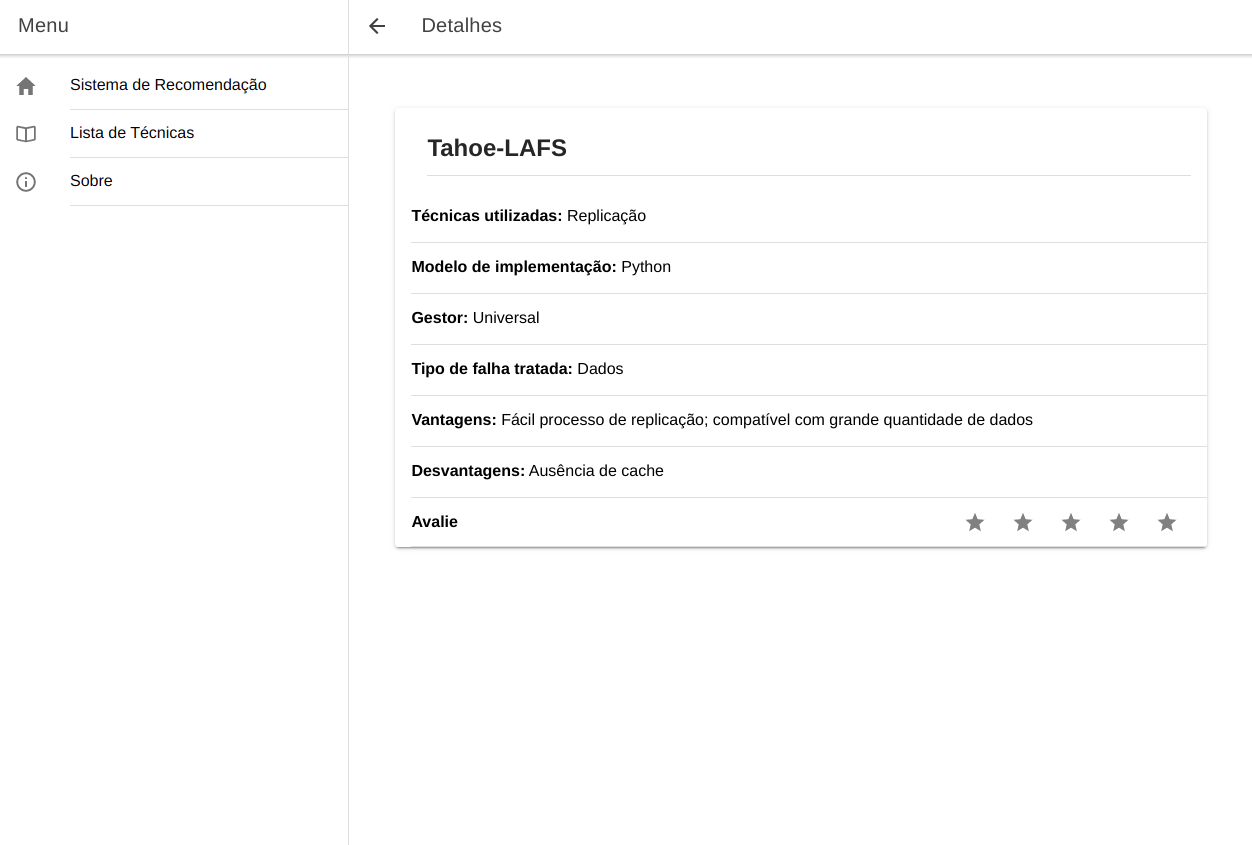
\includegraphics[scale=1.5]{images/sist_recomend2.png}
    \label{fig:sisrec_info}
    \\
\end{figure}

As informações estão dispostas de forma simples e legível para o usuário final, permitindo também que ele volte para a página anterior, e também permitindo a avaliação da técnica em questão para aprimorar as recomendações feitas pelo sistema.

A interface responsiva permite redimensionamento sem perda relevante de dados, como mostrado na figura \ref{fig:sisrec_teste1}, o que a torna apropriada também para dispositivos móveis.

São dispostas 10 recomendaçõs na tela inicial, um número que pode ser alterado dentro do código fonte livremente. O sistema também pode mostrar todas as 52 técnicas cadastrada, como mostrado na figura \ref{fig:tecnicas}.

\begin{figure}
\centering
\begin{minipage}[b]{\textwidth}
  \caption{Tela inicial da ferramenta reduzida}
  \centering
  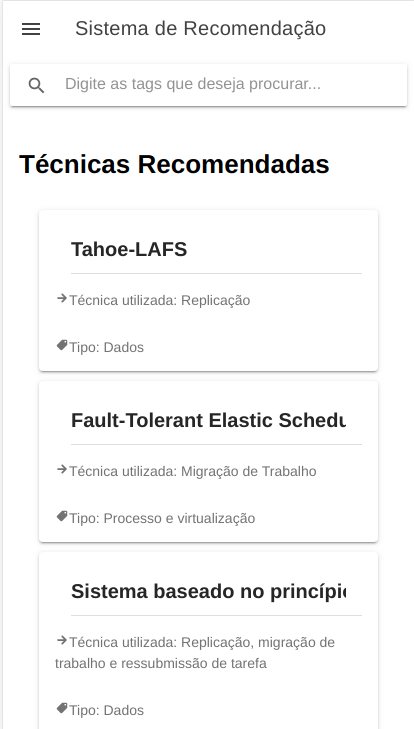
\includegraphics[width=.4\textwidth]{images/sist_recomend1.png}
  \label{fig:sisrec_teste1}
\end{minipage}
\begin{minipage}[b]{\textwidth}
  \centering
  \caption{Tela mostrando uma parcela das técnicas cadastradas}
  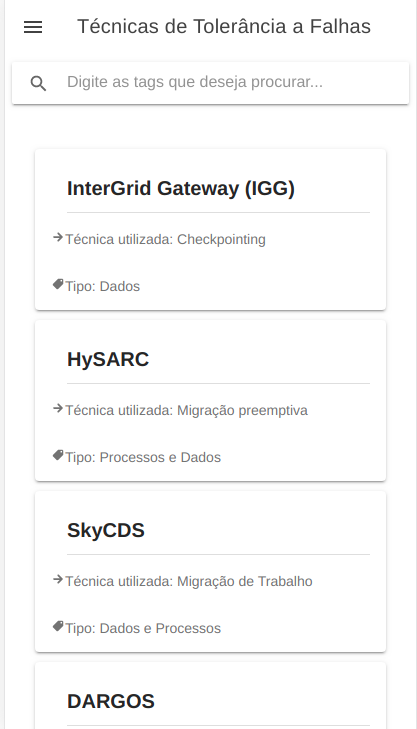
\includegraphics[width=.4\textwidth]{images/tecnicas.png}
  \label{fig:tecnicas}
\end{minipage}
\end{figure}

Nas figuras \ref{fig:filtragem} e \ref{fig:filtragem2} estão demonstradas as funcionalidades de filtragem por escrita da ferramenta. As filtragens podem ser feitas utilizando as principais características das técnicas: o nome, tipo de técnica, modelo de implementação e gestor.

\begin{figure}[H]
\centering
  \begin{subfigure}{\linewidth}
    \caption{Sequência de figuras mostrando a filtragem por modelos de implementação e tipo de técnica, respectivamente}
  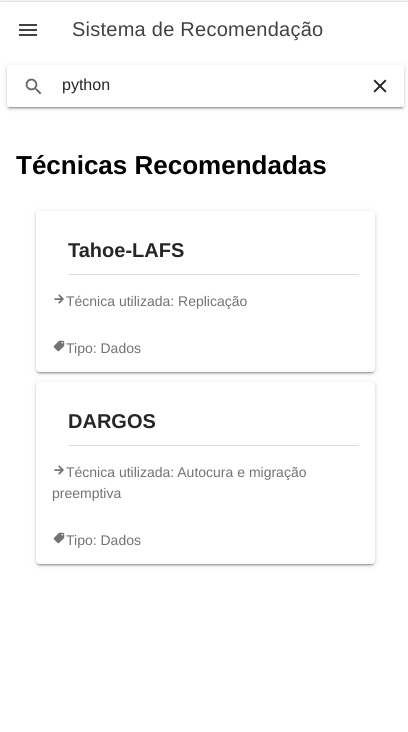
\includegraphics[width=.3\linewidth]{images/filtragem.png}\hfill
  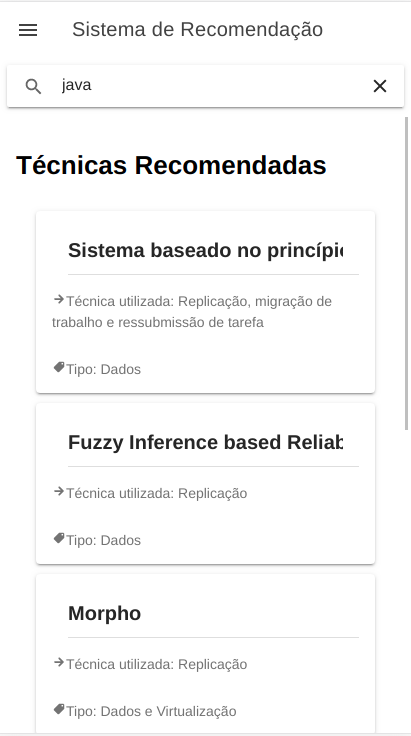
\includegraphics[width=.3\linewidth]{images/filtragem2.png}\hfill
  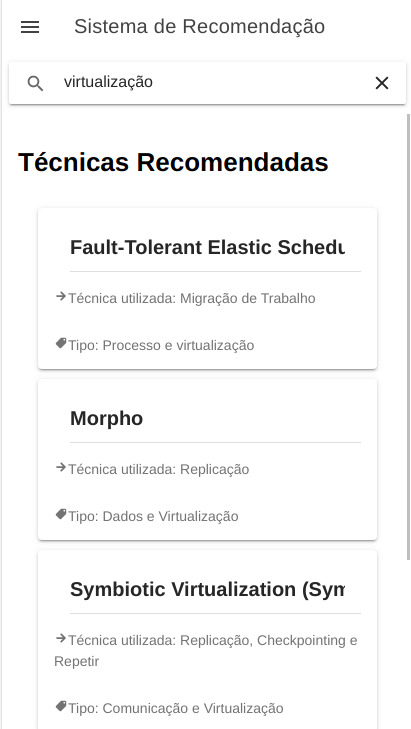
\includegraphics[width=.3\linewidth]{images/filtragem3.png}
  \label{fig:filtragem}
  \end{subfigure}\par\medskip
  \begin{subfigure}{\linewidth}
  \caption{Sequência de figuras mostrando a filtragem por técnica utilizada, nome e gestor, respectivamente}
  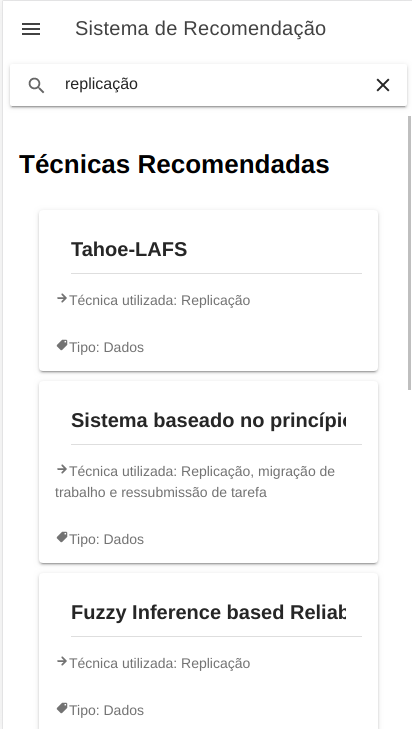
\includegraphics[width=.3\linewidth]{images/filtragem4.png}\hfill
  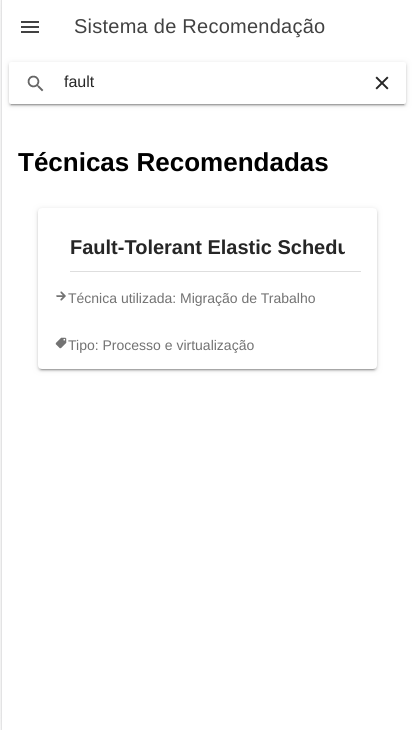
\includegraphics[width=.3\linewidth]{images/filtragem5.png}\hfill
  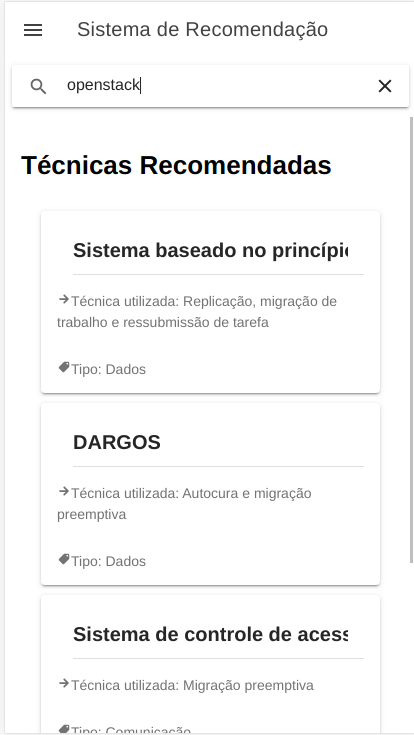
\includegraphics[width=.3\linewidth]{images/filtragem6.png}
  \label{fig:filtragem2}
  \end{subfigure}
\end{figure}

A técnica de filtragem também pode ser utilizada na lista completa de técnicas de tolerância a falhas, funcionando da mesma forma descrita anteriormente.

Para efeito de demonstração da mudança das técnicas recomendadas, na Figura \ref{fig:recomendacoes} estão mostradas diferentes recomendações para diferentes usuários, sob as mesmas condições apresentadas anteriormente.

\begin{figure}[H]
\centering
  \begin{subfigure}{\linewidth}
    \caption{Sequência de figuras mostrando as diferentes recomendações dos usuários com identificador 1, 6 e 10, respectivamente}
  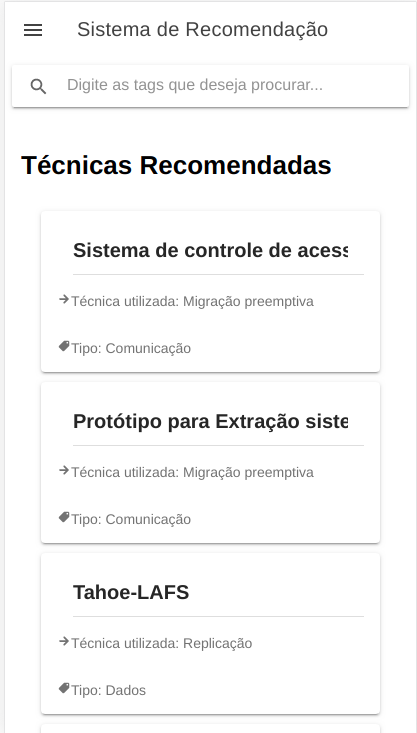
\includegraphics[width=.3\linewidth]{images/recom.png}\hfill
  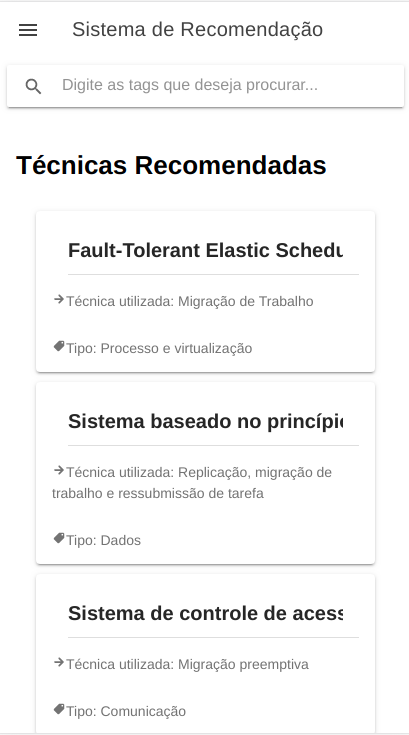
\includegraphics[width=.3\linewidth]{images/recom2.png}\hfill
  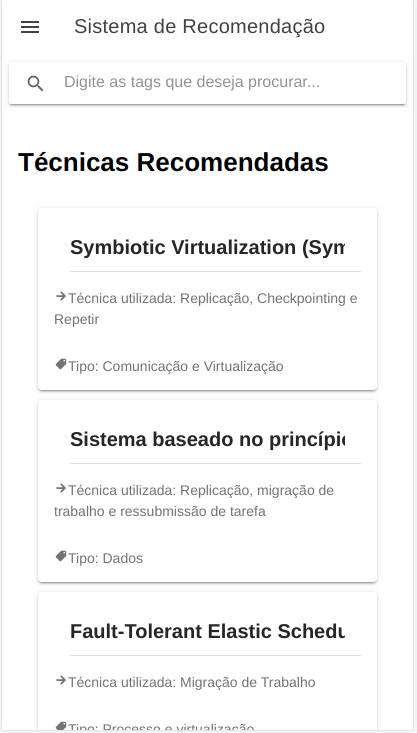
\includegraphics[width=.3\linewidth]{images/recom3.png}
  \label{fig:recomendacoes}
  \end{subfigure}
\end{figure}


\section{Considerações Finais}

Os resultados obtidos dos testes foram bastante satisfatórios, devido ao tamanho do trabalho feito em cima desse projeto e às limitações impostas na tecnologia usada. De maneira geral, o sistema se comporta de forma satisfatória com aquilo que se propõe a fazer, e abre espaço para novas possibilidades com tudo o que já foi implementado. Possui alta flexibilidade e pode ser expandido por terceiros mais tarde, podendo ser até utilizado para outras finalidades.

% ---

% ----------------------------------------------------------
% Finaliza a parte no bookmark do PDF
% para que se inicie o bookmark na raiz
% e adiciona espaço de parte no Sumário
% ----------------------------------------------------------
\phantompart

% ---
% Conclusão
% ---
\chapter{Conclusão} \label{cap_conclusão}
% ---

Neste trabalho foi desenvolvida uma ferramenta que tem como maior atrativo um sistema de recomendação, e que também permite a busca facilitada por meio de caracteres de itens relacionados no arquivo de troca de dados. Pode-se observar que um sistema de recomendação facilita a busca por itens diversos, e possibilita que o usuário se concentre apenas nos dados relevantes para sua pesquisa, sem que a ferramenta o atrapalhe a fazer seu trabalho.

Os resultados obtidos mostram a precisão do modelo do sistema de recomendação desenvolvido neste trabalho, e também comprovam a praticidade e fácil usabilidade do sistema em questão. Esse sistema pode ser livremente utilizado por administradores de sistemas sensíveis a falhas, e deve ser de grande ajuda para os usuários interessados em entender melhor cada tipo de técnica de tolerância a falhas disponível.

Devido à natureza do projeto, ele pode ser posteriormente expandido e também pode ser reaproveitado para outros fins, levando em consideração todas as adaptações feitas para o funcionamento deste projeto. O sistema está disponível para \emph{download} gratuitamente, incluindo o código fonte, instruções para implantação e uma demonstração na página no GitHub (https://github.com/sturdy-robot/sistema-final), sob licença permissiva MIT.




% ----------------------------------------------------------
% ELEMENTOS PÓS-TEXTUAIS
% ----------------------------------------------------------
\postextual
% ----------------------------------------------------------

% ----------------------------------------------------------
% Referências bibliográficas
% ----------------------------------------------------------
\bibliography{referencias}

% ----------------------------------------------------------
% Glossário
% ----------------------------------------------------------
%
% Consulte o manual da classe abntex2 para orientações sobre o glossário.
%
%\glossary

% ----------------------------------------------------------
% Apêndices
% ----------------------------------------------------------

% ---
% Inicia os apêndices
% ---
%\begin{apendicesenv}

% Imprime uma página indicando o início dos apêndices
%\partapendices

% ----------------------------------------------------------
%\chapter{Quisque libero justo}
% ----------------------------------------------------------
%
%\lipsum[50]

%\end{apendicesenv}
% ---


% ----------------------------------------------------------
% Anexos
% ----------------------------------------------------------

% ---
% Inicia os anexos
% ---
%\begin{anexosenv}

% Imprime uma página indicando o início dos anexos
%\partanexos

% ---
%\chapter{Morbi ultrices rutrum lorem.}
% ---
%\lipsum[30]

%\end{anexosenv}

%---------------------------------------------------------------------
% INDICE REMISSIVO
%---------------------------------------------------------------------
\phantompart
\printindex
%---------------------------------------------------------------------

\end{document}
